% Options for packages loaded elsewhere
\PassOptionsToPackage{unicode}{hyperref}
\PassOptionsToPackage{hyphens}{url}
%
\documentclass[
]{article}
\usepackage{amsmath,amssymb}
\usepackage{iftex}
\ifPDFTeX
  \usepackage[T1]{fontenc}
  \usepackage[utf8]{inputenc}
  \usepackage{textcomp} % provide euro and other symbols
\else % if luatex or xetex
  \usepackage{unicode-math} % this also loads fontspec
  \defaultfontfeatures{Scale=MatchLowercase}
  \defaultfontfeatures[\rmfamily]{Ligatures=TeX,Scale=1}
\fi
\usepackage{lmodern}
\ifPDFTeX\else
  % xetex/luatex font selection
\fi
% Use upquote if available, for straight quotes in verbatim environments
\IfFileExists{upquote.sty}{\usepackage{upquote}}{}
\IfFileExists{microtype.sty}{% use microtype if available
  \usepackage[]{microtype}
  \UseMicrotypeSet[protrusion]{basicmath} % disable protrusion for tt fonts
}{}
\makeatletter
\@ifundefined{KOMAClassName}{% if non-KOMA class
  \IfFileExists{parskip.sty}{%
    \usepackage{parskip}
  }{% else
    \setlength{\parindent}{0pt}
    \setlength{\parskip}{6pt plus 2pt minus 1pt}}
}{% if KOMA class
  \KOMAoptions{parskip=half}}
\makeatother
\usepackage{xcolor}
\usepackage[margin=1in]{geometry}
\usepackage{color}
\usepackage{fancyvrb}
\newcommand{\VerbBar}{|}
\newcommand{\VERB}{\Verb[commandchars=\\\{\}]}
\DefineVerbatimEnvironment{Highlighting}{Verbatim}{commandchars=\\\{\}}
% Add ',fontsize=\small' for more characters per line
\usepackage{framed}
\definecolor{shadecolor}{RGB}{248,248,248}
\newenvironment{Shaded}{\begin{snugshade}}{\end{snugshade}}
\newcommand{\AlertTok}[1]{\textcolor[rgb]{0.94,0.16,0.16}{#1}}
\newcommand{\AnnotationTok}[1]{\textcolor[rgb]{0.56,0.35,0.01}{\textbf{\textit{#1}}}}
\newcommand{\AttributeTok}[1]{\textcolor[rgb]{0.13,0.29,0.53}{#1}}
\newcommand{\BaseNTok}[1]{\textcolor[rgb]{0.00,0.00,0.81}{#1}}
\newcommand{\BuiltInTok}[1]{#1}
\newcommand{\CharTok}[1]{\textcolor[rgb]{0.31,0.60,0.02}{#1}}
\newcommand{\CommentTok}[1]{\textcolor[rgb]{0.56,0.35,0.01}{\textit{#1}}}
\newcommand{\CommentVarTok}[1]{\textcolor[rgb]{0.56,0.35,0.01}{\textbf{\textit{#1}}}}
\newcommand{\ConstantTok}[1]{\textcolor[rgb]{0.56,0.35,0.01}{#1}}
\newcommand{\ControlFlowTok}[1]{\textcolor[rgb]{0.13,0.29,0.53}{\textbf{#1}}}
\newcommand{\DataTypeTok}[1]{\textcolor[rgb]{0.13,0.29,0.53}{#1}}
\newcommand{\DecValTok}[1]{\textcolor[rgb]{0.00,0.00,0.81}{#1}}
\newcommand{\DocumentationTok}[1]{\textcolor[rgb]{0.56,0.35,0.01}{\textbf{\textit{#1}}}}
\newcommand{\ErrorTok}[1]{\textcolor[rgb]{0.64,0.00,0.00}{\textbf{#1}}}
\newcommand{\ExtensionTok}[1]{#1}
\newcommand{\FloatTok}[1]{\textcolor[rgb]{0.00,0.00,0.81}{#1}}
\newcommand{\FunctionTok}[1]{\textcolor[rgb]{0.13,0.29,0.53}{\textbf{#1}}}
\newcommand{\ImportTok}[1]{#1}
\newcommand{\InformationTok}[1]{\textcolor[rgb]{0.56,0.35,0.01}{\textbf{\textit{#1}}}}
\newcommand{\KeywordTok}[1]{\textcolor[rgb]{0.13,0.29,0.53}{\textbf{#1}}}
\newcommand{\NormalTok}[1]{#1}
\newcommand{\OperatorTok}[1]{\textcolor[rgb]{0.81,0.36,0.00}{\textbf{#1}}}
\newcommand{\OtherTok}[1]{\textcolor[rgb]{0.56,0.35,0.01}{#1}}
\newcommand{\PreprocessorTok}[1]{\textcolor[rgb]{0.56,0.35,0.01}{\textit{#1}}}
\newcommand{\RegionMarkerTok}[1]{#1}
\newcommand{\SpecialCharTok}[1]{\textcolor[rgb]{0.81,0.36,0.00}{\textbf{#1}}}
\newcommand{\SpecialStringTok}[1]{\textcolor[rgb]{0.31,0.60,0.02}{#1}}
\newcommand{\StringTok}[1]{\textcolor[rgb]{0.31,0.60,0.02}{#1}}
\newcommand{\VariableTok}[1]{\textcolor[rgb]{0.00,0.00,0.00}{#1}}
\newcommand{\VerbatimStringTok}[1]{\textcolor[rgb]{0.31,0.60,0.02}{#1}}
\newcommand{\WarningTok}[1]{\textcolor[rgb]{0.56,0.35,0.01}{\textbf{\textit{#1}}}}
\usepackage{longtable,booktabs,array}
\usepackage{calc} % for calculating minipage widths
% Correct order of tables after \paragraph or \subparagraph
\usepackage{etoolbox}
\makeatletter
\patchcmd\longtable{\par}{\if@noskipsec\mbox{}\fi\par}{}{}
\makeatother
% Allow footnotes in longtable head/foot
\IfFileExists{footnotehyper.sty}{\usepackage{footnotehyper}}{\usepackage{footnote}}
\makesavenoteenv{longtable}
\usepackage{graphicx}
\makeatletter
\def\maxwidth{\ifdim\Gin@nat@width>\linewidth\linewidth\else\Gin@nat@width\fi}
\def\maxheight{\ifdim\Gin@nat@height>\textheight\textheight\else\Gin@nat@height\fi}
\makeatother
% Scale images if necessary, so that they will not overflow the page
% margins by default, and it is still possible to overwrite the defaults
% using explicit options in \includegraphics[width, height, ...]{}
\setkeys{Gin}{width=\maxwidth,height=\maxheight,keepaspectratio}
% Set default figure placement to htbp
\makeatletter
\def\fps@figure{htbp}
\makeatother
\setlength{\emergencystretch}{3em} % prevent overfull lines
\providecommand{\tightlist}{%
  \setlength{\itemsep}{0pt}\setlength{\parskip}{0pt}}
\setcounter{secnumdepth}{5}
\usepackage{pdfpages}
\usepackage{fontspec}
\setmainfont{Times New Roman}
\ifLuaTeX
  \usepackage{selnolig}  % disable illegal ligatures
\fi
\usepackage{bookmark}
\IfFileExists{xurl.sty}{\usepackage{xurl}}{} % add URL line breaks if available
\urlstyle{same}
\hypersetup{
  hidelinks,
  pdfcreator={LaTeX via pandoc}}

\author{}
\date{\vspace{-2.5em}}

\begin{document}

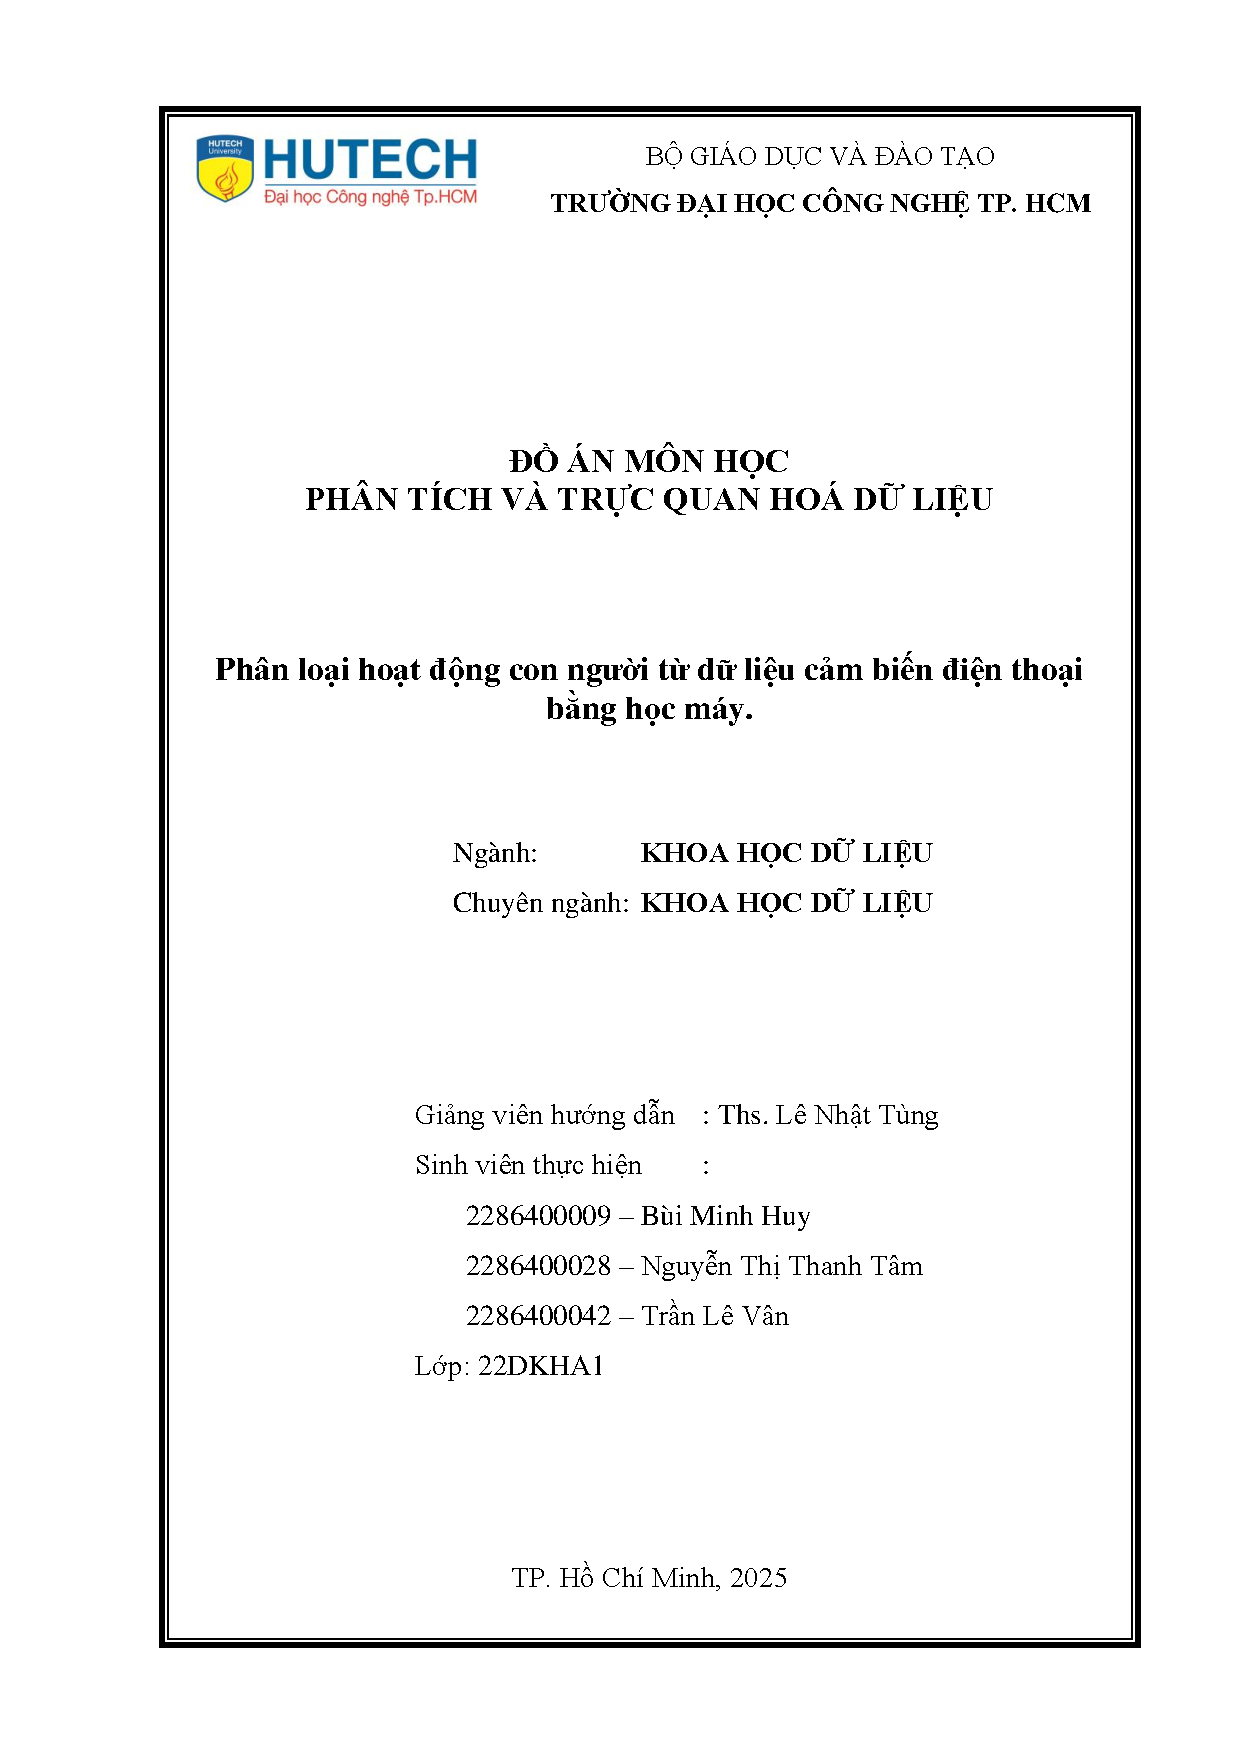
\includepdf[pages=1]{bia.pdf}
\pagenumbering{gobble}

\newpage
\thispagestyle{empty}

\begin{center}
    \LARGE \textbf{LỜI CAM ĐOAN}
\end{center}
\vspace{1.5em}

Chúng tôi, \textbf{Bùi Minh Huy}, \textbf{Trần Lê Vân}, \textbf{Nguyễn
Thị Thanh Tâm} xin cam đoan rằng:

Tất cả thông tin và phân tích trình bày trong báo cáo này được thực hiện
một cách chính xác và trung thực. Mọi dữ liệu, nhận định hoặc ý kiến
được trích dẫn từ các nguồn khác đều đã được nêu rõ nguồn gốc và trích
dẫn đúng quy định. Chúng tôi cam đoan rằng không có bất kỳ hành vi sao
chép hoặc sử dụng thông tin không hợp pháp nào từ các nguồn khác. Bài
báo cáo này là kết quả của công trình nghiên cứu độc lập của chúng tôi
và chưa từng được công bố tại bất kỳ nơi nào khác. Chúng tôi cam đoan đã
tuân thủ nghiêm ngặt các quy tắc và quy định của môn học, bao gồm việc
tham khảo và áp dụng các công cụ nghiên cứu một cách hợp lệ. Nếu phát
hiện có bất kỳ sự gian lận nào, chúng tôi xin hoàn toàn chịu trách nhiệm
về nội dung bài báo cáo của mình. Chúng tôi hy vọng rằng bài báo cáo này
sẽ cung cấp những thông tin hữu ích cho các nhà nghiên cứu, doanh
nghiệp, góp phần vào việc hiểu rõ hơn về mạng xã hội ngày nay.

\vspace{3em}

\begin{flushright}
\begin{minipage}{0.5\textwidth}
\raggedleft
TP.\ Hồ Chí Minh, ngày 28 tháng 3 năm 2025

\vspace{1em}

\centering
\textbf{\LARGE Sinh viên}
\end{minipage}
\end{flushright}

\newpage
\thispagestyle{empty}
\tableofcontents
\newpage
\pagenumbering{arabic}
\setcounter{page}{1}

\section{Abstract}\label{abstract}

\section{Introduction}\label{introduction}

Trong thời đại của điện toán di động và thiết bị thông minh, việc theo
dõi và nhận dạng hoạt động con người (Human Activity Recognition - HAR)
đã trở thành một lĩnh vực nghiên cứu đóng vai trò quan trọng trong nhiều
ngành như trí tuệ nhân tạo, khoa học dữ liệu, y học và công nghệ cảm
biến. HAR đóng vai trò cốt lõi trong các ứng dụng như giám sát sức khỏe,
phát hiện té ngã, điều khiển nhà thông minh. Ngày nay, nhu cầu càng ngày
gia tăng về các thiết bị công nghệ có thể hiểu hành vi con người dẫn đến
việc phát triển các mô hình HAR là chính xác, hiệu quả và có khả năng
triển khai thực tế là vô cùng cần thết.

Một trong những yếu tố chính thúc đẩy sự phát triển của HẢ là sự phổ
biến của các thiết bị di động thông minh và đồng hồ thông minh, vốn đợc
trang bị sẵn các cảm biến quán tính bao gồm gia tốc kế (accelerometer)
và con quay hồi chuyển (gyroscope). Những cảm biến này cho phép thu thập
dữ liệu về chuyển động của người sử dụng với độ chính xác cao, chi phí
thấp và tính khả dụng cao trong đời sống hàng ngày. Nhờ vậy, hệ thống
HAR có thể được lắp đặt mà không cần sử dụng các thiết bị đắt tiền hoặc
lắp đặt phức tạp.

Bên cạnh tiềm năng ứng dụng rộng rãi, việc xây dựng các mô hình HAR vẫn
có nhiều khó khăn thách thức như dữ liệu cảm biến thường có số chiều
lớn, có nhiều dữ liệu nhiễu và có tính biến động cao do phụ thuộc vào
thói quen và hình thể của mỗi người. Bên cạnh đó, một số hoạt động có
thể có mẫu tín hiệu tương tự nhau khiến cho các bài toán phân loại trở
nên khó khăn hơn. Vì vậy, cần có một quy trình xử lý dữ liệu bài bản bao
gồm các bước tiền xử lý dữ liệu, giảm chiều dữ liệu và huấn luyện mô
hình học máy để có thể đặt được hiệu quả cao trong việc nhận dạng hoạt
động con người.

Trong nghiên cứu này, chúng em đã tiến hành khai thác bộ dữ liệu
``\textbf{Human Activity Recognition with Smartphones}'' do UCI Machine
Learning Repository cung cấp, một bộ dữ liệu được sử dụng rộng raix
trong cộng đồng nghiên cứu HAR. Chúng em đề xuất một quy trình học máy
toàn diện bao gồm phân tích đặc trưng, giảm chiều dữ liệu bằng UMAP,
PCA, TSNE và huấn luyện bằng các mô hình học máy như Random Forest,
Decision Tree, Logistic Regression, Support Vectot Machine (SVM) để phân
loại các hoạt động với mục tiêu là nâng cao độ chính xác và hiệu quả của
mô hình. Những kết quả này sẽ cung cấp cái nhìn thực nghiệm rõ ràng cho
các nhà nghiên cứu, đồng thời làm nền móng cho việc triển khai các hệ
thống nhận dạng hoạt động trong thế giới thực.

\section{Dataset and Preprocessing (Dữ liệu và tiền xử
lý)}\label{dataset-and-preprocessing-dux1eef-liux1ec7u-vuxe0-tiux1ec1n-xux1eed-luxfd}

Bộ dữ liệu \textbf{Human Activity Recognition with Smartphones} được thu
thập từ 30 người tham gia (gọi là \emph{subjects}) (15 nam và 15 nữ, độ
tuổi từ 19 đến 48) thực hiện sáu hoạt động thường ngày như Đi bộ
(Walking), đi lên cầu thang (Walking Upstairs), đi xuống cầu thang
(WalkingDownstairs), ngồi (Sitting),đứng (Standing),nằm (Laying). Dữ
liệu được ghi lại bằng một điện thoại thông minh (Samsung Galaxy S II)
đeo ở thắt lưng của người dùng. Các cảm biến gồm \textbf{accelerometer}
và \textbf{gyroscope} được sử dụng để ghi lại chuyển động theo 3 trục X,
Y, Z với tần suất 50Hz.

Mỗi chuỗi tín hiệu được chia thành các \textbf{cửa sổ trượt} có độ dài
2.56 giây, tương ứng với 128 lần đo. Từ mỗi cửa sổ, các đặc trưng
(features) đã được trích xuất từ \textbf{miền thời gian} và \textbf{miền
tần số} để tạo ra một tập hợp dữ liệu có cấu trúc sẵn sàng cho mô hình
học máy.

Các nhóm tín hiệu chính bao gồm:

\begin{itemize}
\tightlist
\item
  \texttt{tBodyAcc-XYZ}: Gia tốc cơ thể theo 3 trục trong miền thời
  gian\\
\item
  \texttt{tGravityAcc-XYZ}: Gia tốc do trọng lực\\
\item
  \texttt{tBodyGyro-XYZ}: Tốc độ quay từ con quay hồi chuyển\\
\item
  \texttt{tBodyAccJerk-XYZ}, \texttt{tBodyGyroJerk-XYZ}: Jerk - đo sự
  thay đổi đột ngột của chuyển động\\
\item
  \texttt{Mag}: Độ lớn vector gia tốc, được tính bằng chuẩn Euclidean:\\
  \[
  \text{Mag} = \sqrt{X^2 + Y^2 + Z^2}
  \]
\item
  \texttt{fBodyAcc-XYZ}, \texttt{fBodyGyro-XYZ}: Biến miền tần số được
  tạo từ FFT
\end{itemize}

Từ các tín hiệu trên, một loạt đặc trưng thống kê được tính toán như:

\begin{itemize}
\item
  \texttt{mean()}, \texttt{std()}, \texttt{mad()}, \texttt{max()},
  \texttt{min()}
\item
  \texttt{sma()}: Signal Magnitude Area
\item
  \texttt{energy()}: Tổng bình phương chia số phần tử
\item
  \texttt{entropy()}, \texttt{iqr()}, \texttt{arCoeff()},
  \texttt{correlation()}
\item
  \texttt{meanFreq()}, \texttt{skewness()}, \texttt{kurtosis()},
  \texttt{bandsEnergy()}, \texttt{angle()}

  Toàn bộ bộ dữ liệu được chia thành hai phần: Tập huấn luyện
  (train.csv): bao gồm 7352 mẫu. Tập kiểm tra (test.csv): bao gồm 2947
  mẫu. Mỗi mẫu tương ứng với một cửa sổ thời gian 2.56 giây, được biểu
  diễn bằng \textbf{561 đặc trưng đầu vào (features)}, 1mỗi mẫu còn bao
  gồm một mã định danh người thực hiện (subject) và một nhãn hoạt động
  (Activity), ác nhãn này được mã hóa từ 1 đến 6 tương ứng với:
\end{itemize}

\begin{longtable}[]{@{}ll@{}}
\toprule\noalign{}
Giá trị nhãn & Hoạt động \\
\midrule\noalign{}
\endhead
\bottomrule\noalign{}
\endlastfoot
1 & WALKING \\
2 & WALKING\_UPSTAIRS \\
3 & WALKING\_DOWNSTAIRS \\
4 & SITTING \\
5 & STANDING \\
6 & LAYING \\
\end{longtable}

\begin{Shaded}
\begin{Highlighting}[]
\CommentTok{\# install.packages("showtext")}
\CommentTok{\# install.packages("ggplot2")}
\end{Highlighting}
\end{Shaded}

\begin{Shaded}
\begin{Highlighting}[]
\CommentTok{\# train \textless{}{-}read.csv(\textquotesingle{}/Users/huy/Documents/doanthaytung/archive/train.csv\textquotesingle{})}
\CommentTok{\# train \textless{}{-}read.csv("D:/BT/clonegit/doanthaytung/archive/train.csv")}
\NormalTok{train }\OtherTok{\textless{}{-}} \FunctionTok{read.csv}\NormalTok{(}\StringTok{\textquotesingle{}archive/train.csv\textquotesingle{}}\NormalTok{)}
\CommentTok{\# head(train)}
\FunctionTok{dim}\NormalTok{(train)}
\end{Highlighting}
\end{Shaded}

\begin{verbatim}
## [1] 7352  563
\end{verbatim}

\begin{Shaded}
\begin{Highlighting}[]
\CommentTok{\# test \textless{}{-}read.csv(\textquotesingle{}/Users/huy/Documents/doanthaytung/archive/test.csv\textquotesingle{})}
\CommentTok{\# test \textless{}{-}read.csv("D:/BT/clonegit/doanthaytung/archive/test.csv")}
\NormalTok{test }\OtherTok{\textless{}{-}} \FunctionTok{read.csv}\NormalTok{(}\StringTok{"archive/test.csv"}\NormalTok{)}
\CommentTok{\# head(test)}
\FunctionTok{dim}\NormalTok{(test)}
\end{Highlighting}
\end{Shaded}

\begin{verbatim}
## [1] 2947  563
\end{verbatim}

xem các các type có trong data

\begin{Shaded}
\begin{Highlighting}[]
\FunctionTok{table}\NormalTok{(}\FunctionTok{sapply}\NormalTok{(train, class))}
\end{Highlighting}
\end{Shaded}

\begin{verbatim}
## 
## character   integer   numeric 
##         1         1       561
\end{verbatim}

in ra cột có dạng charactor

\begin{Shaded}
\begin{Highlighting}[]
\FunctionTok{names}\NormalTok{(train)[}\FunctionTok{sapply}\NormalTok{(train, class) }\SpecialCharTok{==} \StringTok{"character"}\NormalTok{]}
\end{Highlighting}
\end{Shaded}

\begin{verbatim}
## [1] "Activity"
\end{verbatim}

\begin{Shaded}
\begin{Highlighting}[]
\FunctionTok{unique}\NormalTok{(train}\SpecialCharTok{$}\NormalTok{Activity)}
\end{Highlighting}
\end{Shaded}

\begin{verbatim}
## [1] "STANDING"           "SITTING"            "LAYING"            
## [4] "WALKING"            "WALKING_DOWNSTAIRS" "WALKING_UPSTAIRS"
\end{verbatim}

chuyển thành factor

\begin{Shaded}
\begin{Highlighting}[]
\NormalTok{train}\SpecialCharTok{$}\NormalTok{Activity }\OtherTok{\textless{}{-}} \FunctionTok{as.factor}\NormalTok{(train}\SpecialCharTok{$}\NormalTok{Activity)}
\end{Highlighting}
\end{Shaded}

\begin{Shaded}
\begin{Highlighting}[]
\FunctionTok{cat}\NormalTok{(}\StringTok{"Giá trị thiếu ở tập train:"}\NormalTok{, }\FunctionTok{sum}\NormalTok{(}\FunctionTok{is.na}\NormalTok{(train)), }\StringTok{"}\SpecialCharTok{\textbackslash{}n}\StringTok{"}\NormalTok{)}
\end{Highlighting}
\end{Shaded}

\begin{verbatim}
## Giá trị thiếu ở tập train: 0
\end{verbatim}

\begin{Shaded}
\begin{Highlighting}[]
\FunctionTok{cat}\NormalTok{(}\StringTok{"Giá trị thiếu ở tập test:"}\NormalTok{, }\FunctionTok{sum}\NormalTok{(}\FunctionTok{is.na}\NormalTok{(test)), }\StringTok{"}\SpecialCharTok{\textbackslash{}n}\StringTok{"}\NormalTok{)}
\end{Highlighting}
\end{Shaded}

\begin{verbatim}
## Giá trị thiếu ở tập test: 0
\end{verbatim}

\begin{Shaded}
\begin{Highlighting}[]
\FunctionTok{cat}\NormalTok{(}\StringTok{"Số dòng bị trùng lặp trong tập train:"}\NormalTok{, }\FunctionTok{sum}\NormalTok{(}\FunctionTok{duplicated}\NormalTok{(train)), }\StringTok{"}\SpecialCharTok{\textbackslash{}n}\StringTok{"}\NormalTok{)}
\end{Highlighting}
\end{Shaded}

\begin{verbatim}
## Số dòng bị trùng lặp trong tập train: 0
\end{verbatim}

\begin{Shaded}
\begin{Highlighting}[]
\FunctionTok{cat}\NormalTok{(}\StringTok{"Số dòng bị trùng lặp trong tập test :"}\NormalTok{, }\FunctionTok{sum}\NormalTok{(}\FunctionTok{duplicated}\NormalTok{(test)), }\StringTok{"}\SpecialCharTok{\textbackslash{}n}\StringTok{"}\NormalTok{)}
\end{Highlighting}
\end{Shaded}

\begin{verbatim}
## Số dòng bị trùng lặp trong tập test : 0
\end{verbatim}

\begin{Shaded}
\begin{Highlighting}[]
\FunctionTok{library}\NormalTok{(ggplot2)}
\end{Highlighting}
\end{Shaded}

\begin{verbatim}
## Warning: package 'ggplot2' was built under R version 4.4.3
\end{verbatim}

\begin{Shaded}
\begin{Highlighting}[]
\FunctionTok{library}\NormalTok{(showtext)}
\end{Highlighting}
\end{Shaded}

\begin{verbatim}
## Warning: package 'showtext' was built under R version 4.4.3
\end{verbatim}

\begin{verbatim}
## Loading required package: sysfonts
\end{verbatim}

\begin{verbatim}
## Warning: package 'sysfonts' was built under R version 4.4.3
\end{verbatim}

\begin{verbatim}
## Loading required package: showtextdb
\end{verbatim}

\begin{verbatim}
## Warning: package 'showtextdb' was built under R version 4.4.3
\end{verbatim}

\begin{Shaded}
\begin{Highlighting}[]
\FunctionTok{showtext\_auto}\NormalTok{()}

\FunctionTok{ggplot}\NormalTok{(train, }\FunctionTok{aes}\NormalTok{(}\AttributeTok{x =} \FunctionTok{factor}\NormalTok{(subject), }\AttributeTok{fill =}\NormalTok{ Activity)) }\SpecialCharTok{+}
  \FunctionTok{geom\_bar}\NormalTok{(}\AttributeTok{position =} \StringTok{"dodge"}\NormalTok{, }\AttributeTok{width =} \FloatTok{0.7}\NormalTok{) }\SpecialCharTok{+}
  \FunctionTok{scale\_fill\_brewer}\NormalTok{(}\AttributeTok{palette =} \StringTok{"Set2"}\NormalTok{) }\SpecialCharTok{+} 
  \FunctionTok{labs}\NormalTok{(}
    \AttributeTok{title =} \StringTok{"Số lượng mẫu dữ liệu theo người dùng và hoạt động"}\NormalTok{,}
    \AttributeTok{x =} \StringTok{"Người dùng (Subject)"}\NormalTok{,}
    \AttributeTok{y =} \StringTok{"Số lượng mẫu"}\NormalTok{,}
    \AttributeTok{fill =} \StringTok{"Hoạt động"}
\NormalTok{  ) }\SpecialCharTok{+}
  \FunctionTok{theme\_minimal}\NormalTok{(}\AttributeTok{base\_size =} \DecValTok{16}\NormalTok{) }\SpecialCharTok{+}
  \FunctionTok{theme}\NormalTok{(}
    \AttributeTok{plot.title =} \FunctionTok{element\_text}\NormalTok{(}\AttributeTok{hjust =} \FloatTok{0.5}\NormalTok{, }\AttributeTok{face =} \StringTok{"bold"}\NormalTok{, }\AttributeTok{size =} \DecValTok{20}\NormalTok{),}
    \AttributeTok{axis.text.x =} \FunctionTok{element\_text}\NormalTok{(}\AttributeTok{angle =} \DecValTok{45}\NormalTok{, }\AttributeTok{hjust =} \DecValTok{1}\NormalTok{),}
    \AttributeTok{legend.position =} \StringTok{"right"}
\NormalTok{  )}
\end{Highlighting}
\end{Shaded}

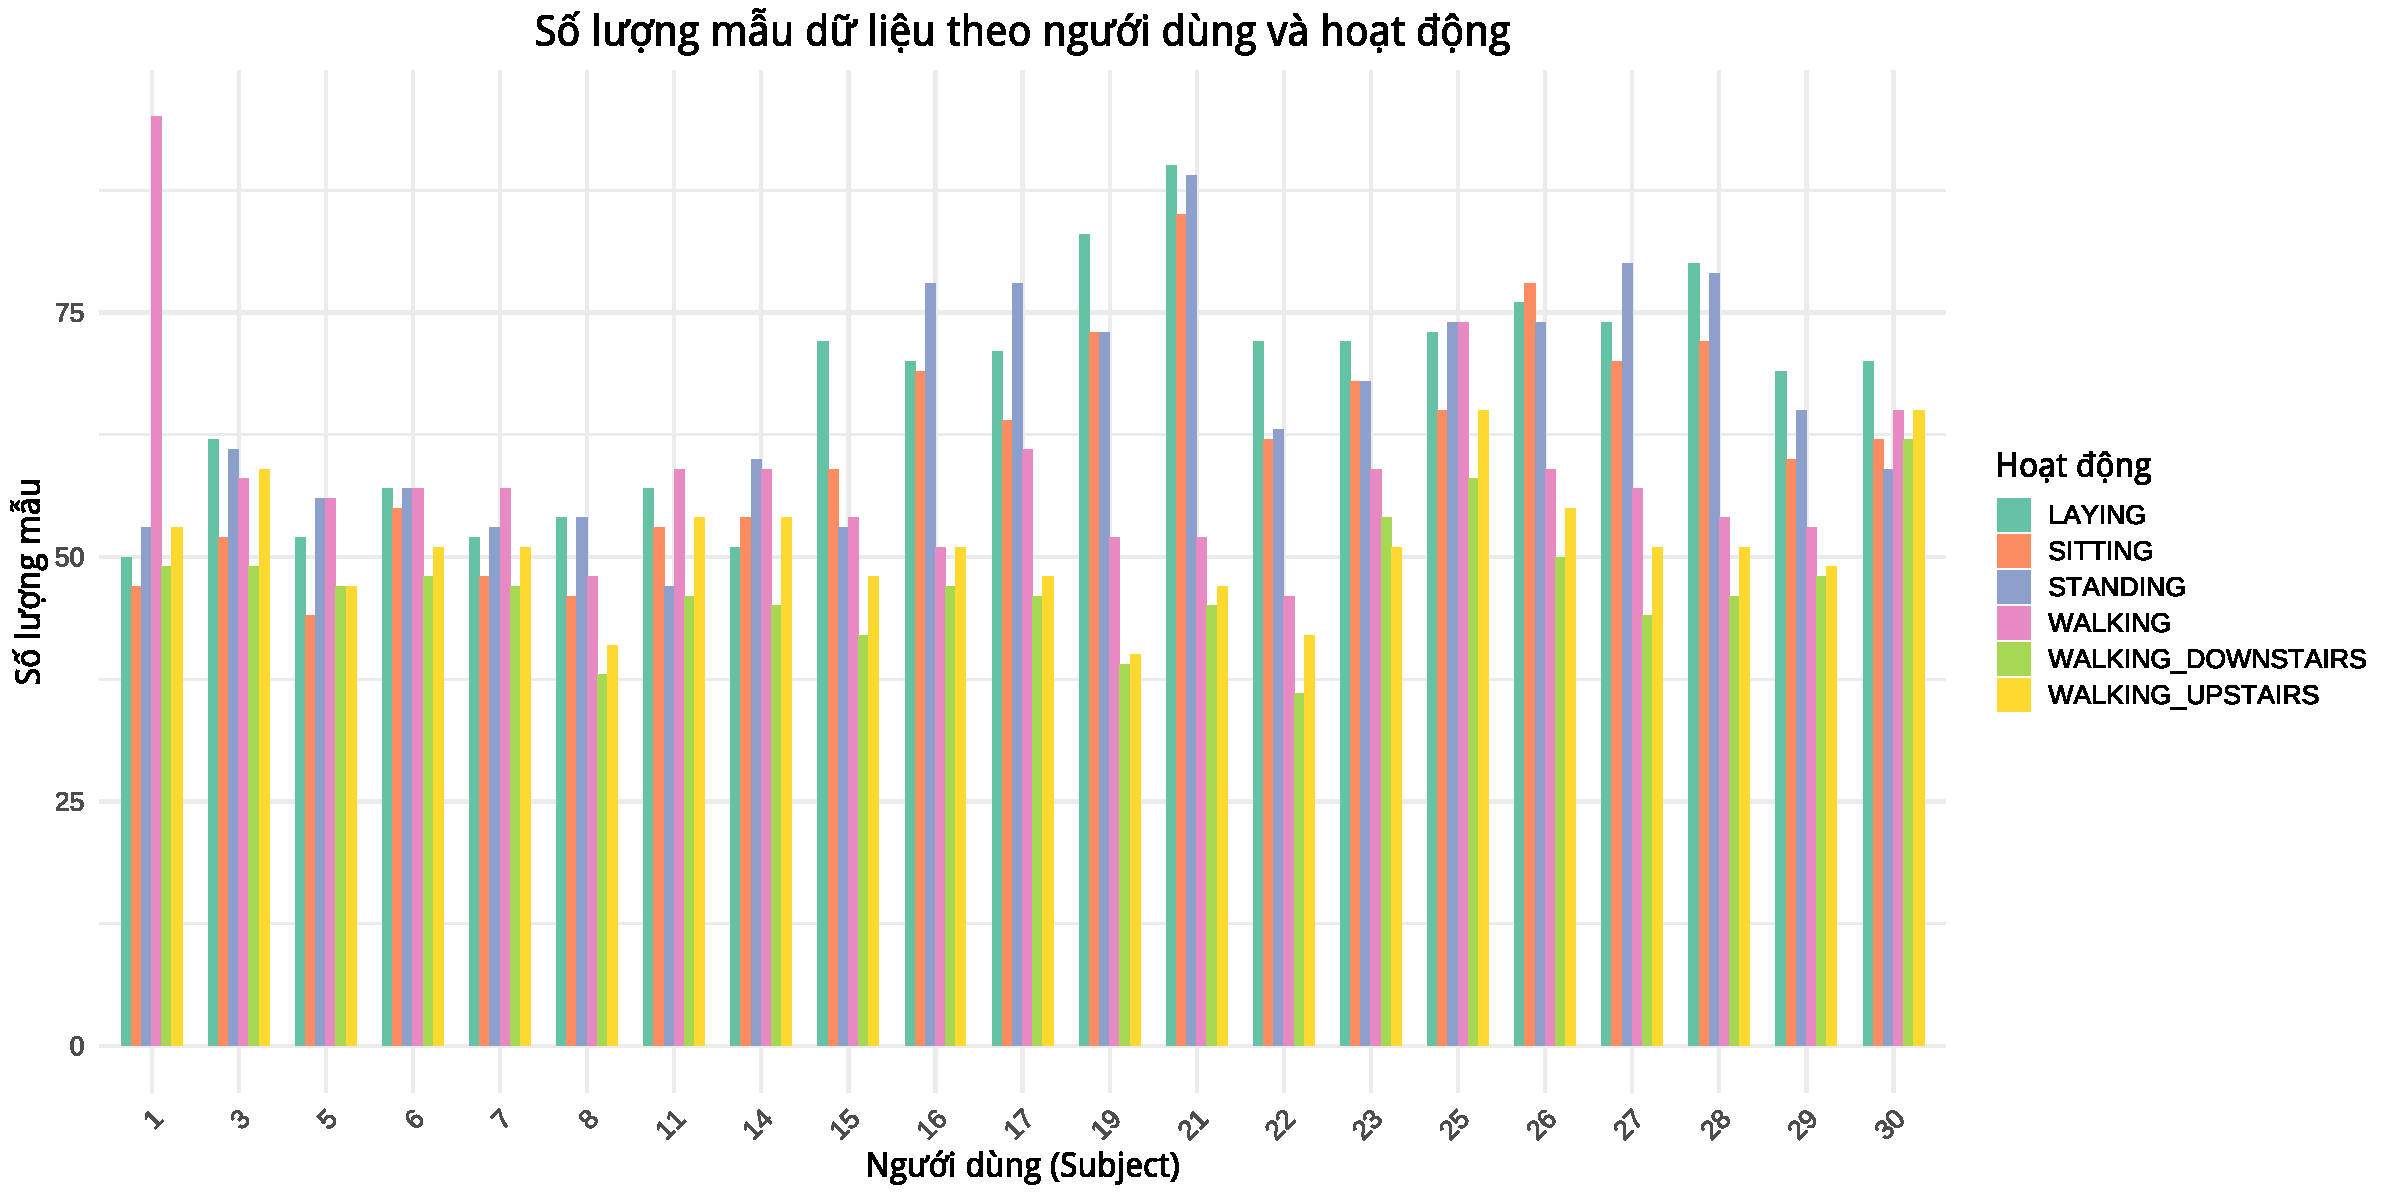
\includegraphics{report_files/figure-latex/unnamed-chunk-10-1.pdf}

\begin{Shaded}
\begin{Highlighting}[]
\FunctionTok{library}\NormalTok{(ggplot2)}

\FunctionTok{ggplot}\NormalTok{(train, }\FunctionTok{aes}\NormalTok{(}\AttributeTok{x =}\NormalTok{ Activity, }\AttributeTok{fill =}\NormalTok{ Activity)) }\SpecialCharTok{+}
  \FunctionTok{geom\_bar}\NormalTok{() }\SpecialCharTok{+}
  \FunctionTok{labs}\NormalTok{(}
    \AttributeTok{title =} \StringTok{"Số lượng mẫu theo từng hoạt động"}\NormalTok{,}
    \AttributeTok{x =} \StringTok{"Hoạt động"}\NormalTok{,}
    \AttributeTok{y =} \StringTok{"Số lượng mẫu"}
\NormalTok{  ) }\SpecialCharTok{+}
  \FunctionTok{theme\_minimal}\NormalTok{(}\AttributeTok{base\_size =} \DecValTok{15}\NormalTok{) }\SpecialCharTok{+}
  \FunctionTok{theme}\NormalTok{(}
    \AttributeTok{axis.text.x =} \FunctionTok{element\_text}\NormalTok{(}\AttributeTok{angle =} \DecValTok{45}\NormalTok{, }\AttributeTok{vjust =} \DecValTok{1}\NormalTok{, }\AttributeTok{hjust=}\DecValTok{1}\NormalTok{),}
    \AttributeTok{plot.title =} \FunctionTok{element\_text}\NormalTok{(}\AttributeTok{hjust =} \FloatTok{0.5}\NormalTok{, }\AttributeTok{face =} \StringTok{"bold"}\NormalTok{)}
\NormalTok{  ) }\SpecialCharTok{+}
  \FunctionTok{guides}\NormalTok{(}\AttributeTok{fill =} \StringTok{"none"}\NormalTok{)}
\end{Highlighting}
\end{Shaded}

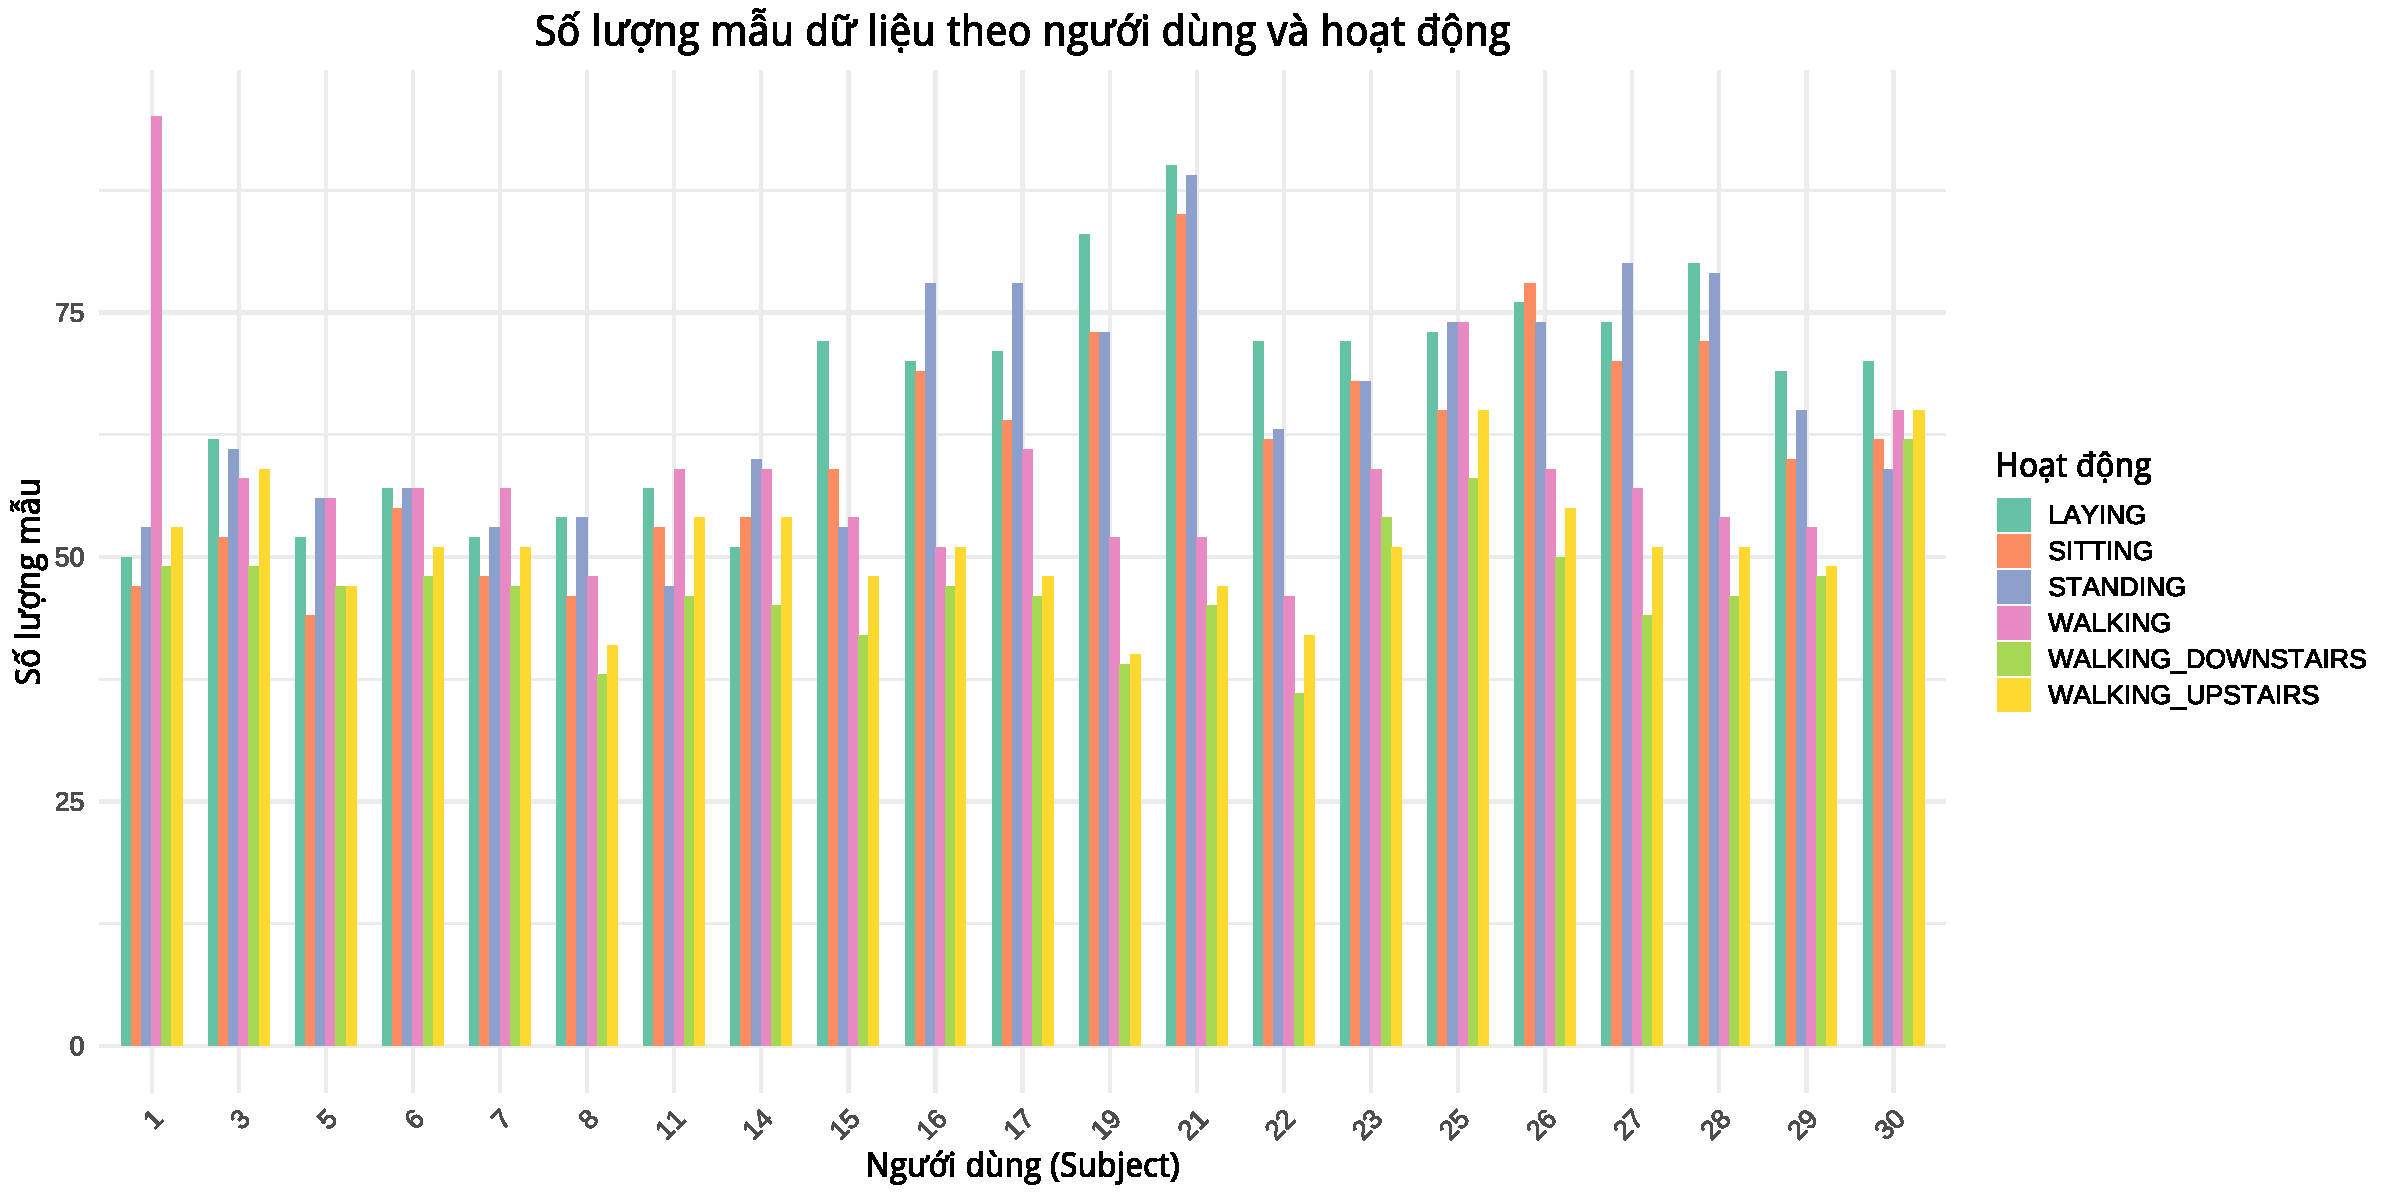
\includegraphics{report_files/figure-latex/unnamed-chunk-11-1.pdf} Số
lượng mẫu cho mỗi hoạt động dao động trong khoảng 1000 mẫu đến 1200 mẫu.
Các hoạt động tĩnh như laying, sitting, standing có xu hướng chiếm tỷ lệ
cao hơn một chút so với các hoạt động di chuyển như walking,
walking\_upstairs, walking\_downstairs. Mức độ chênh lệch không qua lớn
giữa các nhóm, là điểm thuận lợi cho các mô hình học máy tránh bị lệch
nhãn và đảm bảo khả năng học đều giữa các lớp.

\begin{Shaded}
\begin{Highlighting}[]
\NormalTok{columns }\OtherTok{\textless{}{-}} \FunctionTok{colnames}\NormalTok{(train)}
\NormalTok{columns }\OtherTok{\textless{}{-}} \FunctionTok{gsub}\NormalTok{(}\StringTok{"}\SpecialCharTok{\textbackslash{}\textbackslash{}}\StringTok{."}\NormalTok{, }\StringTok{""}\NormalTok{, columns)}
\FunctionTok{colnames}\NormalTok{(train) }\OtherTok{\textless{}{-}}\NormalTok{ columns}
\FunctionTok{colnames}\NormalTok{(test) }\OtherTok{\textless{}{-}}\NormalTok{ columns}
\CommentTok{\# colnames(train)}
\end{Highlighting}
\end{Shaded}

\begin{Shaded}
\begin{Highlighting}[]
\FunctionTok{library}\NormalTok{(ggplot2)}

\FunctionTok{ggplot}\NormalTok{(train, }\FunctionTok{aes}\NormalTok{(}\AttributeTok{x =}\NormalTok{ tBodyAccMagmean, }\AttributeTok{color =}\NormalTok{ Activity)) }\SpecialCharTok{+}
  \FunctionTok{geom\_density}\NormalTok{(}\AttributeTok{size =} \FloatTok{1.2}\NormalTok{) }\SpecialCharTok{+}
  \FunctionTok{scale\_color\_brewer}\NormalTok{(}\AttributeTok{palette =} \StringTok{"Set1"}\NormalTok{) }\SpecialCharTok{+}
  \FunctionTok{scale\_x\_continuous}\NormalTok{(}\AttributeTok{limits =} \FunctionTok{c}\NormalTok{(}\SpecialCharTok{{-}}\FloatTok{1.1}\NormalTok{, }\DecValTok{1}\NormalTok{)) }\SpecialCharTok{+} 
  \FunctionTok{labs}\NormalTok{(}
    \AttributeTok{title =} \StringTok{"Phân bố tBodyAccMagmean theo hoạt động"}\NormalTok{,}
    \AttributeTok{x =} \StringTok{"tBodyAccMagmean"}\NormalTok{,}
    \AttributeTok{y =} \StringTok{"Mật độ"}
\NormalTok{  ) }\SpecialCharTok{+}
  \FunctionTok{theme\_minimal}\NormalTok{(}\AttributeTok{base\_size =} \DecValTok{16}\NormalTok{) }\SpecialCharTok{+}
  \FunctionTok{theme}\NormalTok{(}
    \AttributeTok{plot.title =} \FunctionTok{element\_text}\NormalTok{(}\AttributeTok{hjust =} \FloatTok{0.5}\NormalTok{)}
\NormalTok{  )}
\end{Highlighting}
\end{Shaded}

\begin{verbatim}
## Warning: Using `size` aesthetic for lines was deprecated in ggplot2 3.4.0.
## i Please use `linewidth` instead.
## This warning is displayed once every 8 hours.
## Call `lifecycle::last_lifecycle_warnings()` to see where this warning was
## generated.
\end{verbatim}

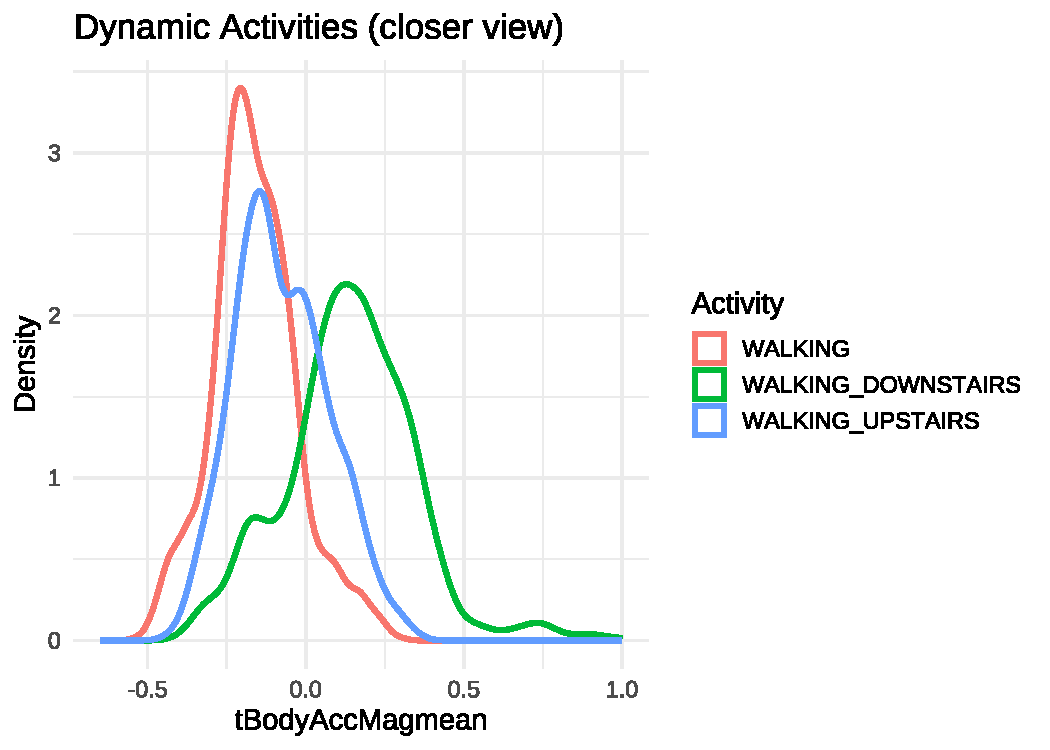
\includegraphics{report_files/figure-latex/unnamed-chunk-13-1.pdf}

\begin{Shaded}
\begin{Highlighting}[]
\FunctionTok{class}\NormalTok{(train}\SpecialCharTok{$}\NormalTok{Activity)}
\end{Highlighting}
\end{Shaded}

\begin{verbatim}
## [1] "factor"
\end{verbatim}

\begin{Shaded}
\begin{Highlighting}[]
\FunctionTok{unique}\NormalTok{(train}\SpecialCharTok{$}\NormalTok{Activity)}
\end{Highlighting}
\end{Shaded}

\begin{verbatim}
## [1] STANDING           SITTING            LAYING             WALKING           
## [5] WALKING_DOWNSTAIRS WALKING_UPSTAIRS  
## 6 Levels: LAYING SITTING STANDING WALKING ... WALKING_UPSTAIRS
\end{verbatim}

\begin{Shaded}
\begin{Highlighting}[]
\FunctionTok{library}\NormalTok{(ggplot2)}
\FunctionTok{library}\NormalTok{(dplyr)}
\end{Highlighting}
\end{Shaded}

\begin{verbatim}
## 
## Attaching package: 'dplyr'
\end{verbatim}

\begin{verbatim}
## The following objects are masked from 'package:stats':
## 
##     filter, lag
\end{verbatim}

\begin{verbatim}
## The following objects are masked from 'package:base':
## 
##     intersect, setdiff, setequal, union
\end{verbatim}

\begin{Shaded}
\begin{Highlighting}[]
\FunctionTok{library}\NormalTok{(gridExtra)}
\end{Highlighting}
\end{Shaded}

\begin{verbatim}
## 
## Attaching package: 'gridExtra'
\end{verbatim}

\begin{verbatim}
## The following object is masked from 'package:dplyr':
## 
##     combine
\end{verbatim}

\begin{Shaded}
\begin{Highlighting}[]
\NormalTok{p1 }\OtherTok{\textless{}{-}}\NormalTok{ train }\SpecialCharTok{\%\textgreater{}\%}
  \FunctionTok{filter}\NormalTok{(Activity }\SpecialCharTok{\%in\%} \FunctionTok{c}\NormalTok{(}\StringTok{"SITTING"}\NormalTok{, }\StringTok{"STANDING"}\NormalTok{, }\StringTok{"LAYING"}\NormalTok{)) }\SpecialCharTok{\%\textgreater{}\%}
  \FunctionTok{ggplot}\NormalTok{(}\FunctionTok{aes}\NormalTok{(}\AttributeTok{x =}\NormalTok{ tBodyAccMagmean, }\AttributeTok{color =}\NormalTok{ Activity)) }\SpecialCharTok{+}
  \FunctionTok{geom\_density}\NormalTok{(}\AttributeTok{size =} \FloatTok{1.2}\NormalTok{) }\SpecialCharTok{+}
  \FunctionTok{labs}\NormalTok{(}
    \AttributeTok{title =} \StringTok{"Static Activities (closer view)"}\NormalTok{,}
    \AttributeTok{x =} \StringTok{"tBodyAccMagmean"}\NormalTok{,}
    \AttributeTok{y =} \StringTok{"Density"}
\NormalTok{  ) }\SpecialCharTok{+}
  \FunctionTok{xlim}\NormalTok{(}\SpecialCharTok{{-}}\FloatTok{1.05}\NormalTok{, }\SpecialCharTok{{-}}\FloatTok{0.1}\NormalTok{) }\SpecialCharTok{+}
  \FunctionTok{ylim}\NormalTok{(}\DecValTok{0}\NormalTok{, }\DecValTok{35}\NormalTok{) }\SpecialCharTok{+}
  \FunctionTok{theme\_minimal}\NormalTok{(}\AttributeTok{base\_size =} \DecValTok{14}\NormalTok{)}
\NormalTok{p1}
\end{Highlighting}
\end{Shaded}

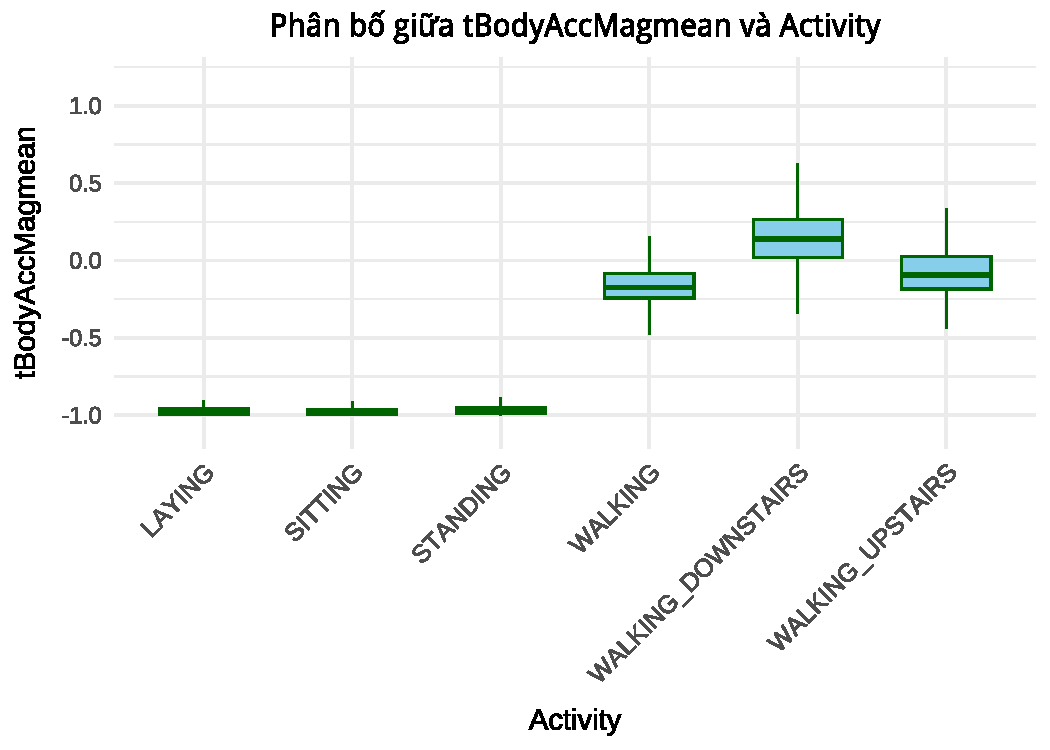
\includegraphics{report_files/figure-latex/unnamed-chunk-16-1.pdf}

\begin{Shaded}
\begin{Highlighting}[]
\NormalTok{p2 }\OtherTok{\textless{}{-}}\NormalTok{ train }\SpecialCharTok{\%\textgreater{}\%}
  \FunctionTok{filter}\NormalTok{(Activity }\SpecialCharTok{\%in\%} \FunctionTok{c}\NormalTok{(}\StringTok{"WALKING"}\NormalTok{, }\StringTok{"WALKING\_DOWNSTAIRS"}\NormalTok{, }\StringTok{"WALKING\_UPSTAIRS"}\NormalTok{)) }\SpecialCharTok{\%\textgreater{}\%}
  \FunctionTok{ggplot}\NormalTok{(}\FunctionTok{aes}\NormalTok{(}\AttributeTok{x =}\NormalTok{ tBodyAccMagmean, }\AttributeTok{color =}\NormalTok{ Activity)) }\SpecialCharTok{+}
  \FunctionTok{geom\_density}\NormalTok{(}\AttributeTok{size =} \FloatTok{1.2}\NormalTok{) }\SpecialCharTok{+}
  \FunctionTok{labs}\NormalTok{(}
    \AttributeTok{title =} \StringTok{"Dynamic Activities (closer view)"}\NormalTok{,}
    \AttributeTok{x =} \StringTok{"tBodyAccMagmean"}\NormalTok{,}
    \AttributeTok{y =} \StringTok{"Density"}
\NormalTok{  ) }\SpecialCharTok{+} \FunctionTok{xlim}\NormalTok{(}\SpecialCharTok{{-}}\FloatTok{0.65}\NormalTok{, }\DecValTok{1}\NormalTok{) }\SpecialCharTok{+}
  \FunctionTok{theme\_minimal}\NormalTok{(}\AttributeTok{base\_size =} \DecValTok{14}\NormalTok{)}

\NormalTok{p2}
\end{Highlighting}
\end{Shaded}

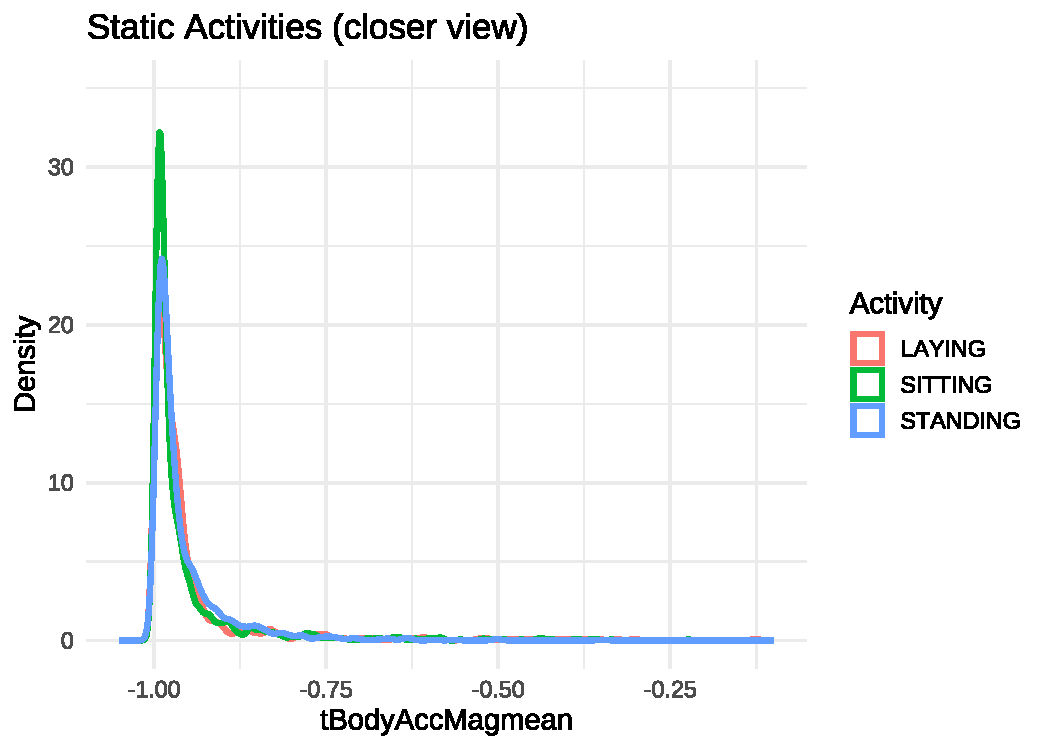
\includegraphics{report_files/figure-latex/unnamed-chunk-17-1.pdf}

\begin{Shaded}
\begin{Highlighting}[]
\FunctionTok{library}\NormalTok{(ggplot2)}

\FunctionTok{ggplot}\NormalTok{(train, }\FunctionTok{aes}\NormalTok{(}\AttributeTok{x =}\NormalTok{ Activity, }\AttributeTok{y =}\NormalTok{ tBodyAccMagmean)) }\SpecialCharTok{+}
  \FunctionTok{geom\_boxplot}\NormalTok{(}
    \AttributeTok{outlier.shape =} \ConstantTok{NA}\NormalTok{,}
    \AttributeTok{fill =} \StringTok{"skyblue"}\NormalTok{,}
    \AttributeTok{color =} \StringTok{"darkgreen"}\NormalTok{,}
    \AttributeTok{width =} \FloatTok{0.6}
\NormalTok{  ) }\SpecialCharTok{+}
  \FunctionTok{labs}\NormalTok{(}
    \AttributeTok{title =} \StringTok{"Phân bố giữa tBodyAccMagmean và Activity"}\NormalTok{,}
    \AttributeTok{y =} \StringTok{"tBodyAccMagmean"}\NormalTok{,}
    \AttributeTok{x =} \StringTok{"Activity"}
\NormalTok{  ) }\SpecialCharTok{+}
  \FunctionTok{coord\_cartesian}\NormalTok{(}\AttributeTok{ylim =} \FunctionTok{c}\NormalTok{(}\SpecialCharTok{{-}}\FloatTok{1.1}\NormalTok{, }\FloatTok{1.2}\NormalTok{)) }\SpecialCharTok{+} 
  \FunctionTok{theme\_minimal}\NormalTok{(}\AttributeTok{base\_size =} \DecValTok{14}\NormalTok{) }\SpecialCharTok{+}
  \FunctionTok{theme}\NormalTok{(}
    \AttributeTok{plot.title =} \FunctionTok{element\_text}\NormalTok{(}\AttributeTok{hjust =} \FloatTok{0.5}\NormalTok{, }\AttributeTok{size =} \DecValTok{15}\NormalTok{, }\AttributeTok{face =} \StringTok{"bold"}\NormalTok{),}
    \AttributeTok{axis.text.x =} \FunctionTok{element\_text}\NormalTok{(}\AttributeTok{angle =} \DecValTok{45}\NormalTok{, }\AttributeTok{hjust =} \DecValTok{1}\NormalTok{, }\AttributeTok{size =} \DecValTok{12}\NormalTok{),}
    \AttributeTok{axis.title.x =} \FunctionTok{element\_text}\NormalTok{(}\AttributeTok{margin =} \FunctionTok{margin}\NormalTok{(}\AttributeTok{t =} \DecValTok{10}\NormalTok{)),}
    \AttributeTok{axis.title.y =} \FunctionTok{element\_text}\NormalTok{(}\AttributeTok{margin =} \FunctionTok{margin}\NormalTok{(}\AttributeTok{r =} \DecValTok{10}\NormalTok{))}
\NormalTok{  )}
\end{Highlighting}
\end{Shaded}

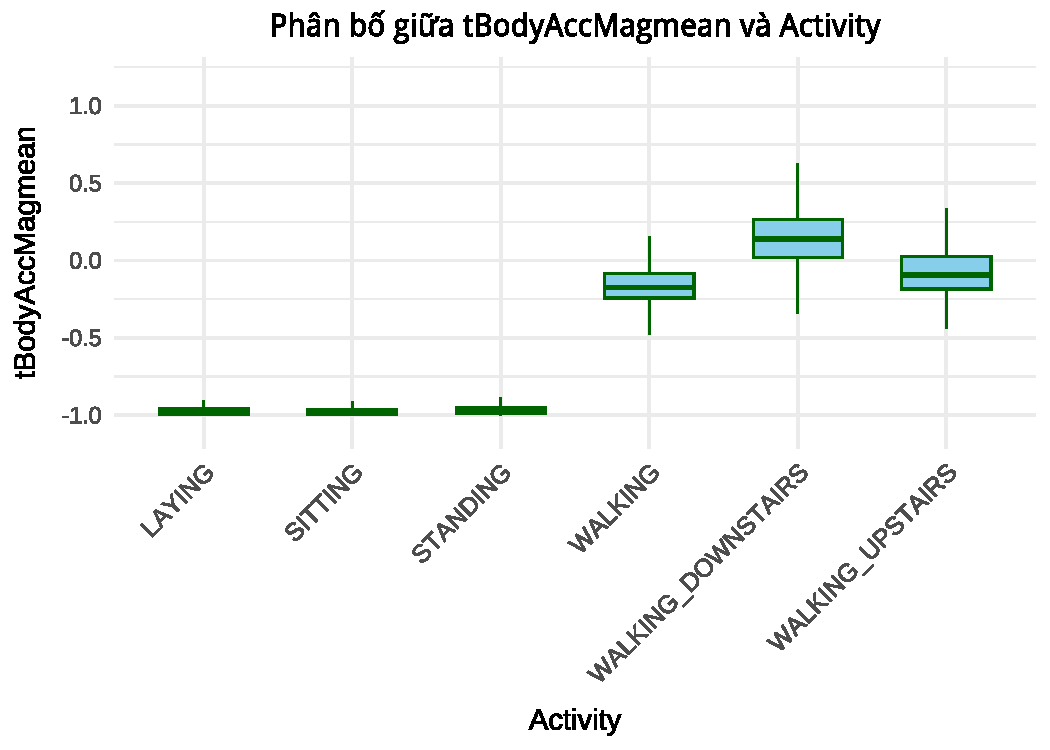
\includegraphics{report_files/figure-latex/unnamed-chunk-18-1.pdf}

\begin{Shaded}
\begin{Highlighting}[]
\FunctionTok{library}\NormalTok{(ggplot2)}

\FunctionTok{ggplot}\NormalTok{(train, }\FunctionTok{aes}\NormalTok{(}\AttributeTok{x =}\NormalTok{ Activity, }\AttributeTok{y =}\NormalTok{ angleXgravityMean)) }\SpecialCharTok{+}
  \FunctionTok{geom\_boxplot}\NormalTok{(}
    \AttributeTok{fill =} \StringTok{"lightblue"}\NormalTok{,}
    \AttributeTok{color =} \StringTok{"darkblue"}\NormalTok{,}
    \AttributeTok{outlier.shape =} \ConstantTok{NA}\NormalTok{,}
    \AttributeTok{width =} \FloatTok{0.6}
\NormalTok{  ) }\SpecialCharTok{+}
  \FunctionTok{labs}\NormalTok{(}
    \AttributeTok{title =} \StringTok{"Phân bố giữa angleXgravityMean và Activity"}\NormalTok{,}
    \AttributeTok{x =} \StringTok{"Activity"}\NormalTok{,}
    \AttributeTok{y =} \StringTok{"angleXgravityMean"}
\NormalTok{  ) }\SpecialCharTok{+}
  \FunctionTok{theme\_minimal}\NormalTok{(}\AttributeTok{base\_size =} \DecValTok{14}\NormalTok{) }\SpecialCharTok{+}
  \FunctionTok{theme}\NormalTok{(}
    \AttributeTok{plot.title =} \FunctionTok{element\_text}\NormalTok{(}\AttributeTok{hjust =} \FloatTok{0.5}\NormalTok{, }\AttributeTok{size =} \DecValTok{15}\NormalTok{, }\AttributeTok{face =} \StringTok{"bold"}\NormalTok{),}
    \AttributeTok{axis.text.x =} \FunctionTok{element\_text}\NormalTok{(}\AttributeTok{angle =} \DecValTok{40}\NormalTok{, }\AttributeTok{hjust =} \DecValTok{1}\NormalTok{, }\AttributeTok{size =} \DecValTok{11}\NormalTok{)}
\NormalTok{  )}
\end{Highlighting}
\end{Shaded}

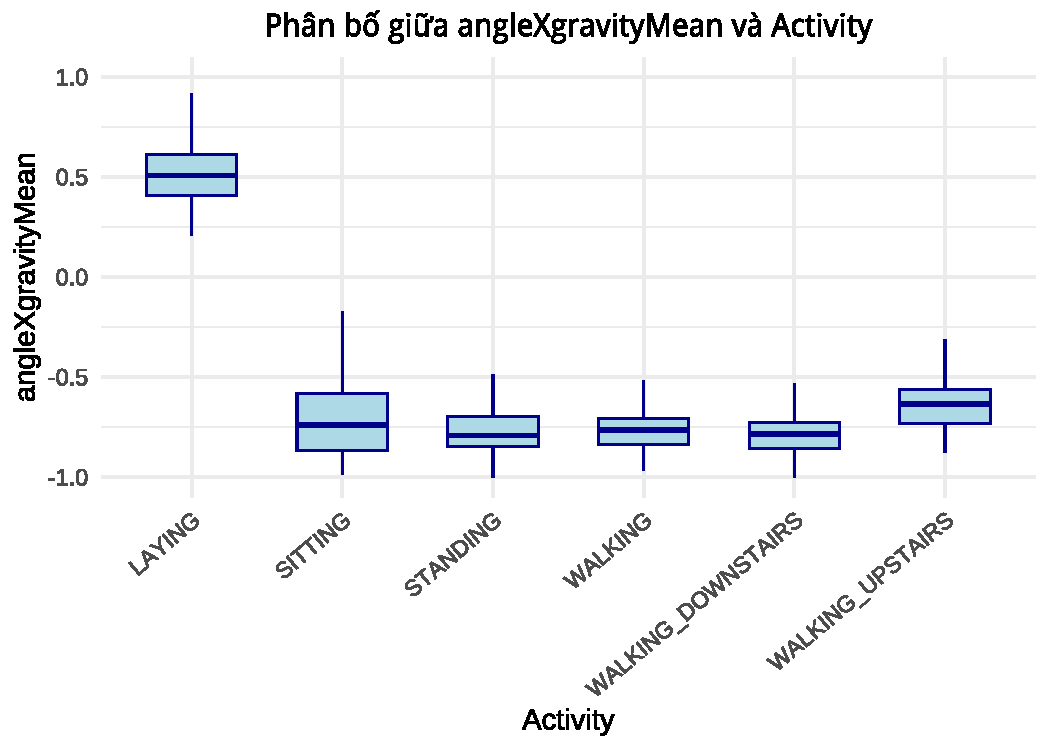
\includegraphics{report_files/figure-latex/unnamed-chunk-19-1.pdf}

\begin{Shaded}
\begin{Highlighting}[]
\FunctionTok{library}\NormalTok{(ggplot2)}

\FunctionTok{ggplot}\NormalTok{(train, }\FunctionTok{aes}\NormalTok{(}\AttributeTok{x =}\NormalTok{ Activity, }\AttributeTok{y =}\NormalTok{ angleYgravityMean)) }\SpecialCharTok{+}
  \FunctionTok{geom\_boxplot}\NormalTok{(}
    \AttributeTok{fill =} \StringTok{"lightblue"}\NormalTok{,}
    \AttributeTok{color =} \StringTok{"darkblue"}\NormalTok{,}
    \AttributeTok{outlier.shape =} \ConstantTok{NA}\NormalTok{,}
    \AttributeTok{width =} \FloatTok{0.6}
\NormalTok{  ) }\SpecialCharTok{+}
  \FunctionTok{labs}\NormalTok{(}
    \AttributeTok{title =} \StringTok{"Phân bố giữa angleYgravityMean và Activity"}\NormalTok{,}
    \AttributeTok{x =} \StringTok{"Activity"}\NormalTok{,}
    \AttributeTok{y =} \StringTok{"angleYgravityMean"}
\NormalTok{  ) }\SpecialCharTok{+}
  \FunctionTok{theme\_minimal}\NormalTok{(}\AttributeTok{base\_size =} \DecValTok{14}\NormalTok{) }\SpecialCharTok{+}
  \FunctionTok{theme}\NormalTok{(}
    \AttributeTok{plot.title =} \FunctionTok{element\_text}\NormalTok{(}\AttributeTok{hjust =} \FloatTok{0.5}\NormalTok{, }\AttributeTok{size =} \DecValTok{15}\NormalTok{, }\AttributeTok{face =} \StringTok{"bold"}\NormalTok{),}
    \AttributeTok{axis.text.x =} \FunctionTok{element\_text}\NormalTok{(}\AttributeTok{angle =} \DecValTok{40}\NormalTok{, }\AttributeTok{hjust =} \DecValTok{1}\NormalTok{, }\AttributeTok{size =} \DecValTok{11}\NormalTok{)}
\NormalTok{  )}
\end{Highlighting}
\end{Shaded}

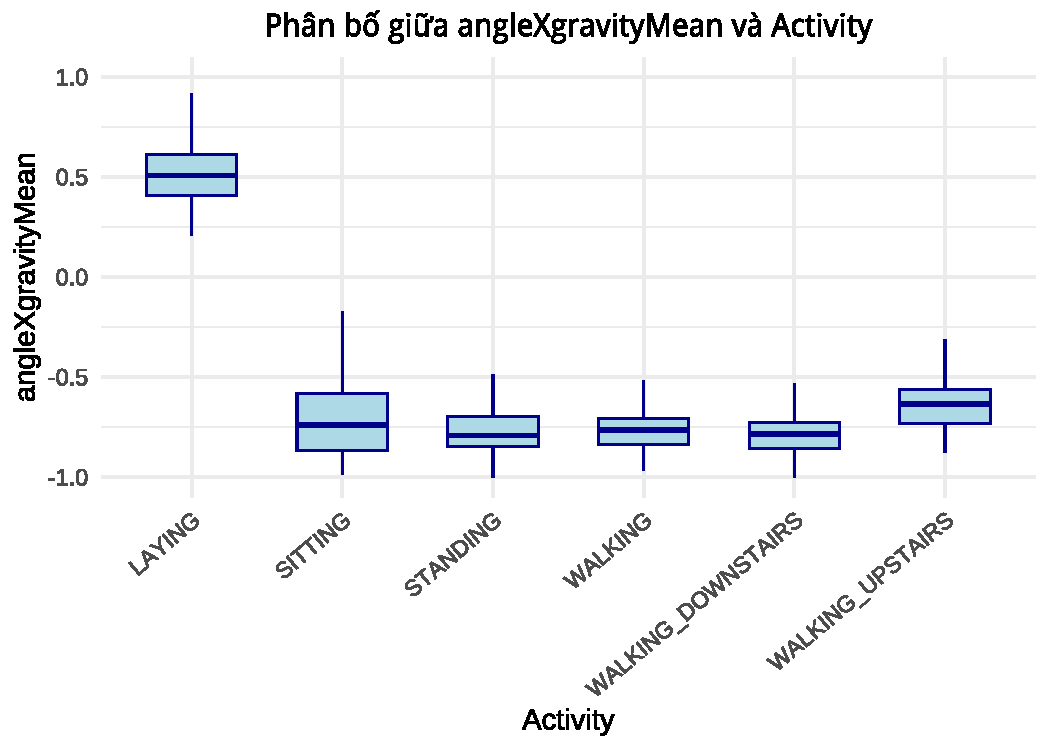
\includegraphics{report_files/figure-latex/unnamed-chunk-20-1.pdf}

\textbf{Kmean}

\begin{Shaded}
\begin{Highlighting}[]
\NormalTok{train\_kmean }\OtherTok{\textless{}{-}}\NormalTok{ train}
\NormalTok{X }\OtherTok{\textless{}{-}}\NormalTok{ train\_kmean  }\SpecialCharTok{\%\textgreater{}\%} \FunctionTok{select}\NormalTok{(}\SpecialCharTok{{-}}\NormalTok{Activity, }\SpecialCharTok{{-}}\NormalTok{subject)}
\NormalTok{wcss }\OtherTok{\textless{}{-}} \FunctionTok{numeric}\NormalTok{(}\DecValTok{10}\NormalTok{)}
\ControlFlowTok{for}\NormalTok{(i }\ControlFlowTok{in} \DecValTok{1}\SpecialCharTok{:}\DecValTok{10}\NormalTok{) \{}
\NormalTok{  kmeans\_model }\OtherTok{\textless{}{-}} \FunctionTok{kmeans}\NormalTok{(X, }\AttributeTok{centers=}\NormalTok{i, }\AttributeTok{nstart=}\DecValTok{25}\NormalTok{)}
\NormalTok{  wcss[i]  }\OtherTok{\textless{}{-}}\NormalTok{ kmeans\_model}\SpecialCharTok{$}\NormalTok{tot.withinss}
\NormalTok{\}}

\FunctionTok{plot}\NormalTok{(}\DecValTok{1}\SpecialCharTok{:}\DecValTok{10}\NormalTok{, wcss, }\AttributeTok{type =} \StringTok{"b"}\NormalTok{, }\AttributeTok{pch =} \DecValTok{19}\NormalTok{, }
     \AttributeTok{xlab =} \StringTok{"Số cụm (K)"}\NormalTok{, }
     \AttributeTok{ylab =} \StringTok{"Tổng bình phương khoảng cách trong cụm (WCSS)"}\NormalTok{,}
     \AttributeTok{main =} \StringTok{"Phương pháp Elbow"}\NormalTok{)}
\end{Highlighting}
\end{Shaded}

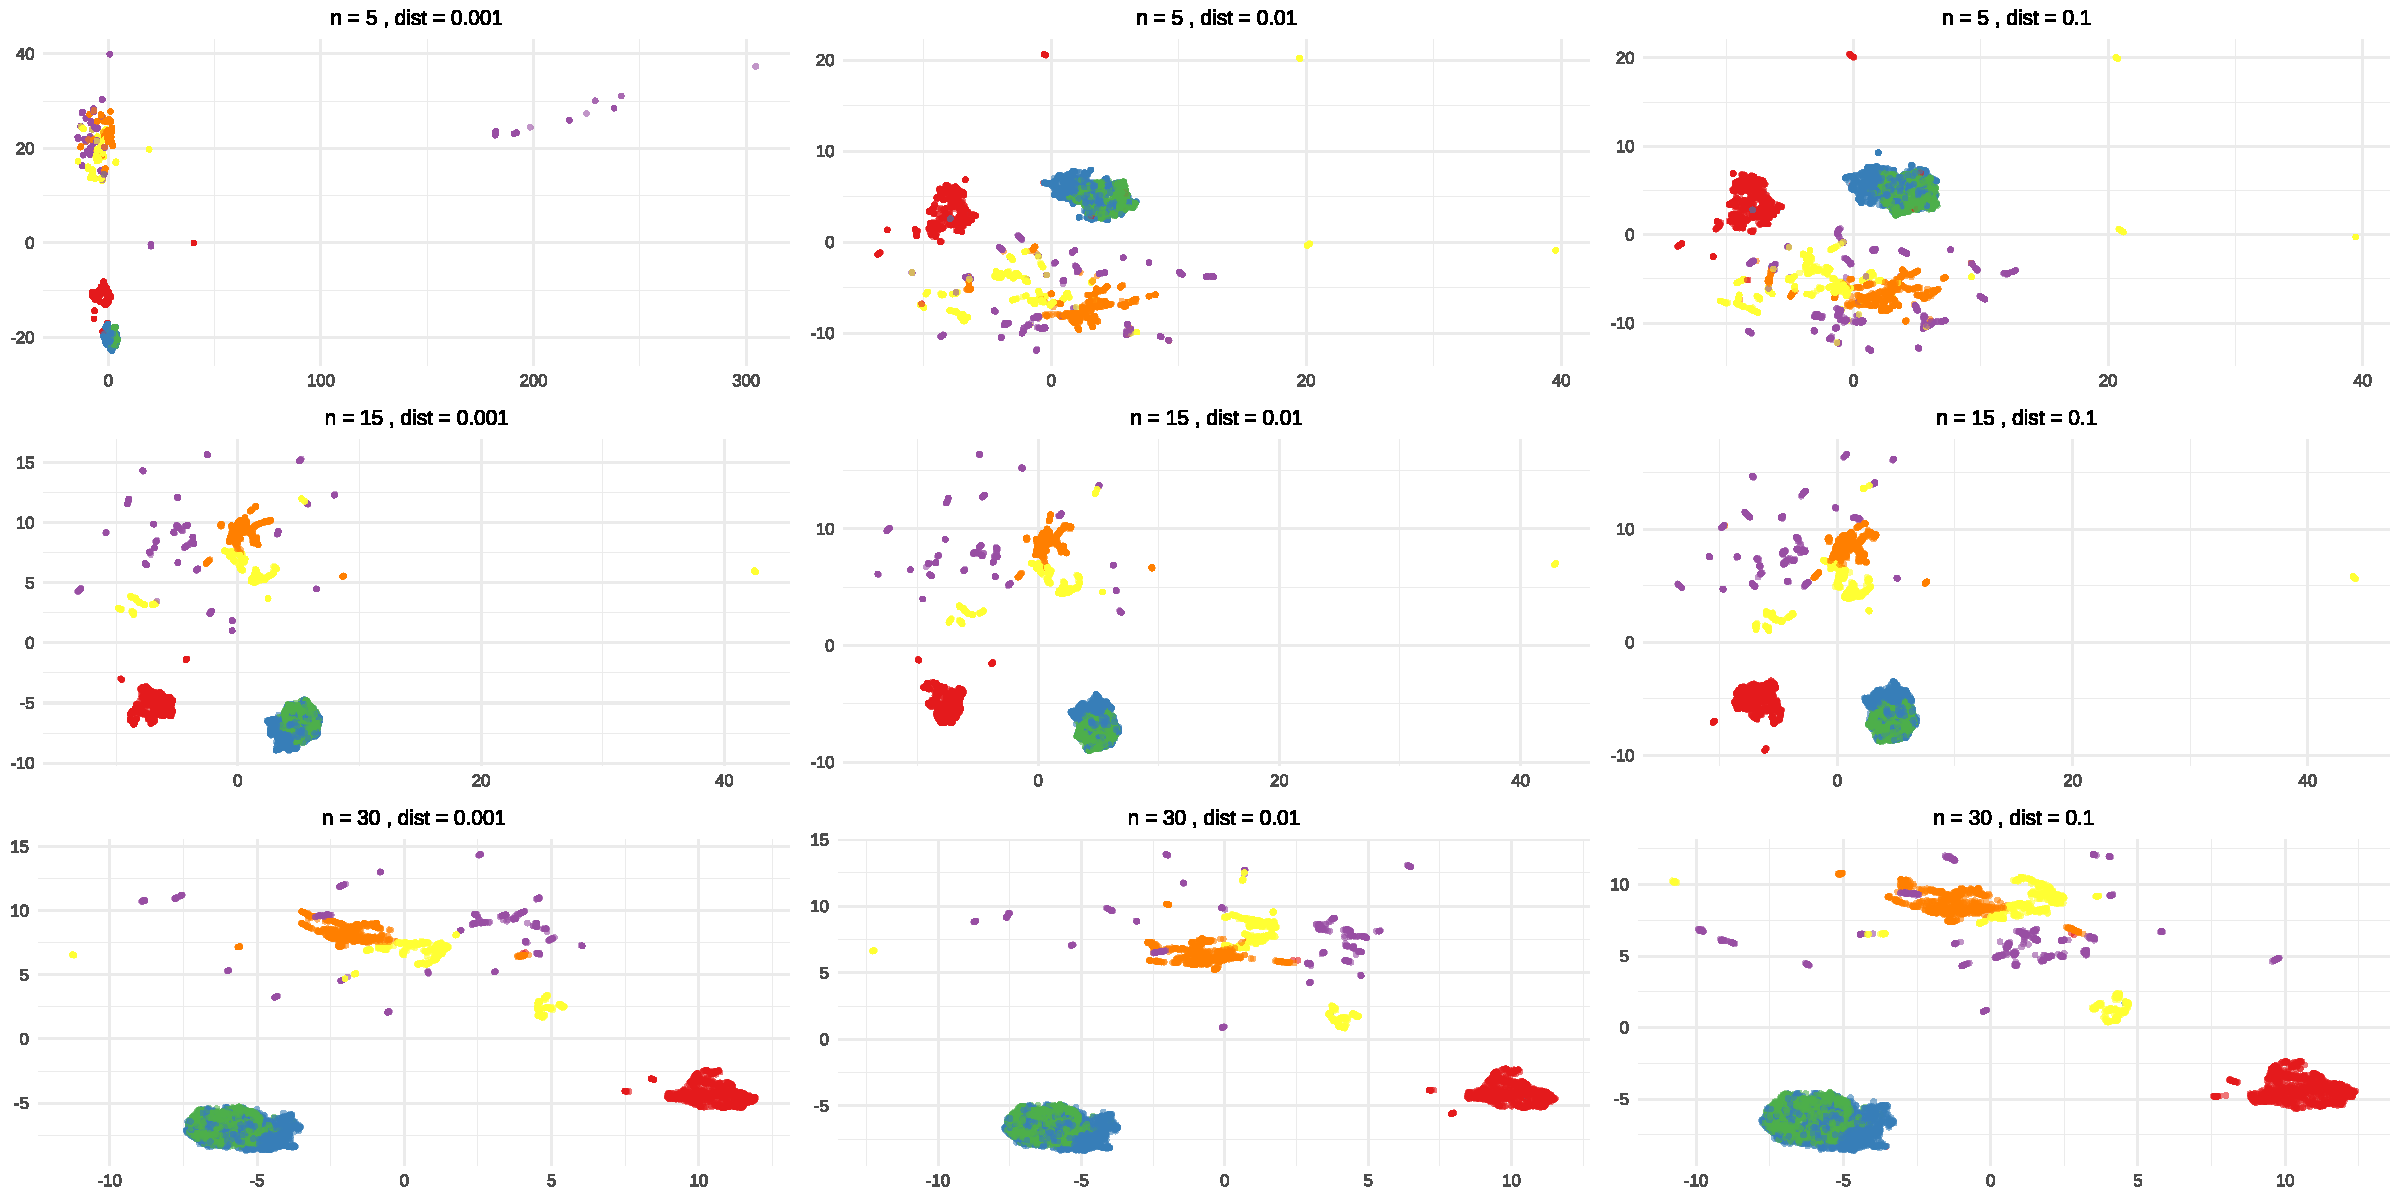
\includegraphics{report_files/figure-latex/unnamed-chunk-21-1.pdf}

\begin{Shaded}
\begin{Highlighting}[]
\CommentTok{\# \# Tính điểm Silhouette trung bình cho các giá trị K từ 2 đến 10}
\CommentTok{\# library(cluster)}
\CommentTok{\# }
\CommentTok{\# avg\_sil \textless{}{-} numeric(9)}
\CommentTok{\# for(k in 2:10) \{}
\CommentTok{\#   km \textless{}{-} kmeans(X, centers = k, nstart = 25)}
\CommentTok{\#   ss \textless{}{-} silhouette(km$cluster, dist(X))}
\CommentTok{\#   avg\_sil[k{-}1] \textless{}{-} mean(ss[, 3])}
\CommentTok{\# \}}
\CommentTok{\# }
\CommentTok{\# \# Vẽ biểu đồ Silhouette}
\CommentTok{\# plot(2:10, avg\_sil, type = "b", pch = 19,}
\CommentTok{\#      xlab = "So luong cum (K)",}
\CommentTok{\#      ylab = "Diem Silhouette trung binh",}
\CommentTok{\#      main = "Phuong phap Silhouette")}
\end{Highlighting}
\end{Shaded}

Đánh giá kết quả phân cụm với k = 2

\begin{Shaded}
\begin{Highlighting}[]
\FunctionTok{library}\NormalTok{(factoextra)}
\end{Highlighting}
\end{Shaded}

\begin{verbatim}
## Warning: package 'factoextra' was built under R version 4.4.3
\end{verbatim}

\begin{verbatim}
## Welcome! Want to learn more? See two factoextra-related books at https://goo.gl/ve3WBa
\end{verbatim}

\begin{Shaded}
\begin{Highlighting}[]
\FunctionTok{library}\NormalTok{(cluster)}

\CommentTok{\# Áp dụng K{-}Means với K = 2}
\NormalTok{km\_result }\OtherTok{\textless{}{-}} \FunctionTok{kmeans}\NormalTok{(X, }\AttributeTok{centers =} \DecValTok{2}\NormalTok{, }\AttributeTok{nstart =} \DecValTok{100}\NormalTok{)}

\CommentTok{\# Tính và vẽ biểu đồ Silhouette}
\NormalTok{sil }\OtherTok{\textless{}{-}} \FunctionTok{silhouette}\NormalTok{(km\_result}\SpecialCharTok{$}\NormalTok{cluster, }\FunctionTok{dist}\NormalTok{(X))}
\FunctionTok{fviz\_silhouette}\NormalTok{(sil, }\AttributeTok{print.summary =} \ConstantTok{TRUE}\NormalTok{)}
\end{Highlighting}
\end{Shaded}

\begin{verbatim}
##   cluster size ave.sil.width
## 1       1 4055          0.52
## 2       2 3297          0.45
\end{verbatim}

\begin{figure}
\centering
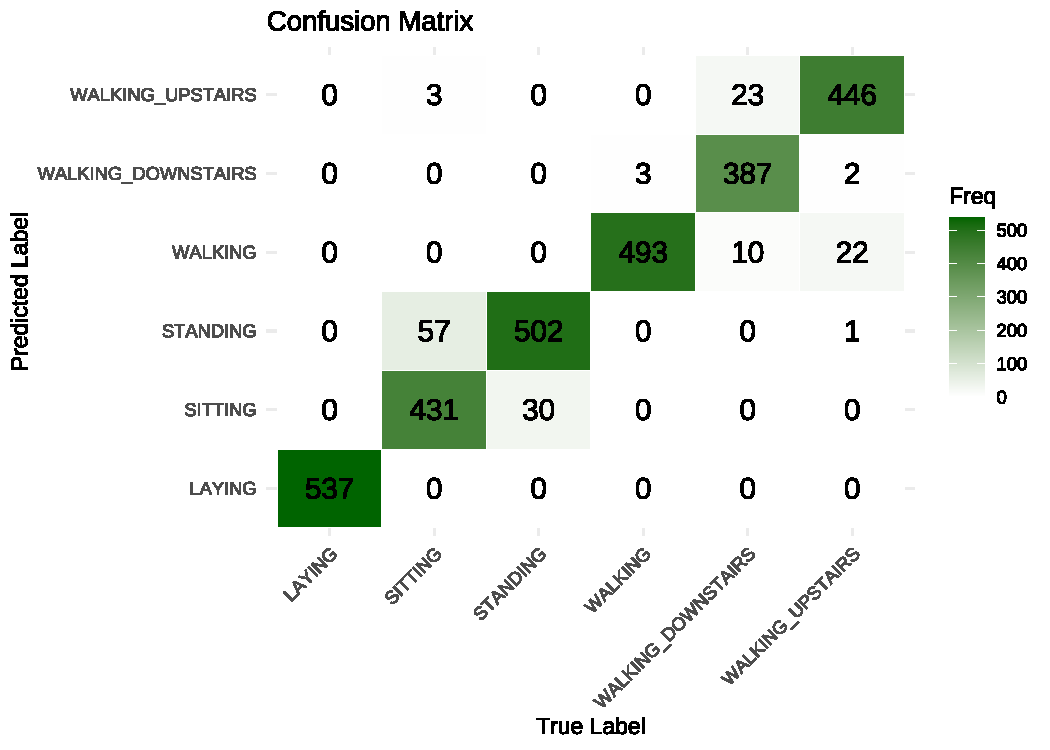
\includegraphics{report_files/figure-latex/unnamed-chunk-23-1.pdf}
\caption{Bieu do Silhouette cho ket qua phan cum}
\end{figure}

Trực quan kết quả phân cụm với k = 2

\begin{Shaded}
\begin{Highlighting}[]
\NormalTok{label\_cluster }\OtherTok{\textless{}{-}} \FunctionTok{ifelse}\NormalTok{(km\_result}\SpecialCharTok{$}\NormalTok{cluster }\SpecialCharTok{==} \DecValTok{1}\NormalTok{, }\StringTok{"Tĩnh"}\NormalTok{, }\StringTok{"Di chuyển"}\NormalTok{)}
\NormalTok{km\_labeled }\OtherTok{\textless{}{-}}\NormalTok{ km\_result}
\NormalTok{km\_labeled}\SpecialCharTok{$}\NormalTok{cluster }\OtherTok{\textless{}{-}} \FunctionTok{as.factor}\NormalTok{(label\_cluster)}
\FunctionTok{fviz\_cluster}\NormalTok{(km\_labeled, }\AttributeTok{data =}\NormalTok{ X,}
             \AttributeTok{palette =} \FunctionTok{c}\NormalTok{(}\StringTok{"\#1B9E77"}\NormalTok{, }\StringTok{"\#D95F02"}\NormalTok{),}
             \AttributeTok{geom =} \StringTok{"point"}\NormalTok{,}
             \AttributeTok{ellipse.type =} \StringTok{"convex"}\NormalTok{,}
             \AttributeTok{ggtheme =} \FunctionTok{theme\_minimal}\NormalTok{(),}
             \AttributeTok{main =} \StringTok{"Ket qua phan cum K{-}Means (K=2)"}\NormalTok{)}
\end{Highlighting}
\end{Shaded}

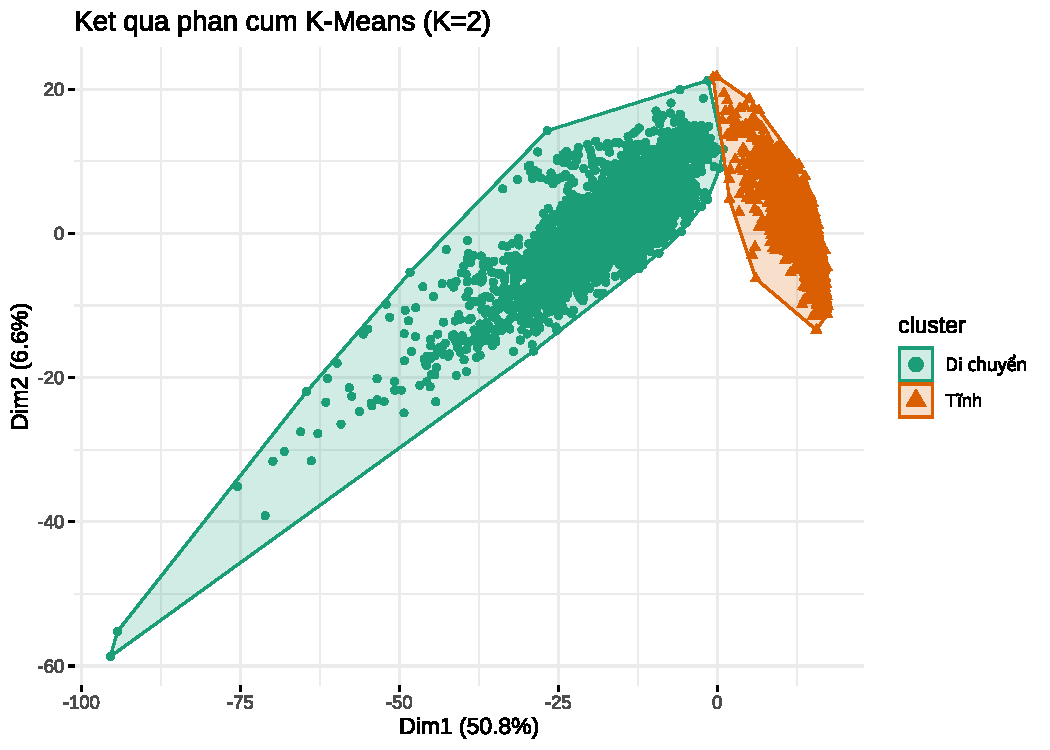
\includegraphics{report_files/figure-latex/unnamed-chunk-24-1.pdf}

\begin{Shaded}
\begin{Highlighting}[]
\NormalTok{train\_pca }\OtherTok{\textless{}{-}}\NormalTok{ train  }
\NormalTok{df\_pca }\OtherTok{\textless{}{-}}\NormalTok{ train\_pca }\SpecialCharTok{\%\textgreater{}\%} \FunctionTok{select}\NormalTok{(}\SpecialCharTok{{-}}\NormalTok{subject, }\SpecialCharTok{{-}}\NormalTok{Activity)}
\NormalTok{pca\_result }\OtherTok{\textless{}{-}} \FunctionTok{prcomp}\NormalTok{(df\_pca, }\AttributeTok{center =} \ConstantTok{TRUE}\NormalTok{, }\AttributeTok{scale. =} \ConstantTok{TRUE}\NormalTok{)}
\NormalTok{df\_pca\_result }\OtherTok{\textless{}{-}} \FunctionTok{as.data.frame}\NormalTok{(pca\_result}\SpecialCharTok{$}\NormalTok{x[, }\DecValTok{1}\SpecialCharTok{:}\DecValTok{2}\NormalTok{])  }
\NormalTok{df\_pca\_result}\SpecialCharTok{$}\NormalTok{Activity }\OtherTok{\textless{}{-}}\NormalTok{ train}\SpecialCharTok{$}\NormalTok{Activity  }

\CommentTok{\# df\_pca\_result}
\end{Highlighting}
\end{Shaded}

\begin{Shaded}
\begin{Highlighting}[]
\FunctionTok{ggplot}\NormalTok{(df\_pca\_result, }\FunctionTok{aes}\NormalTok{(}\AttributeTok{x =}\NormalTok{ PC1, }\AttributeTok{y =}\NormalTok{ PC2, }\AttributeTok{color =}\NormalTok{ Activity)) }\SpecialCharTok{+}
  \FunctionTok{geom\_point}\NormalTok{(}\AttributeTok{alpha =} \FloatTok{0.7}\NormalTok{) }\SpecialCharTok{+}
  \FunctionTok{labs}\NormalTok{(}
    \AttributeTok{title =} \StringTok{" PCA "}\NormalTok{,}
    \AttributeTok{x =} \StringTok{"Thành phần chính 1 (PC1)"}\NormalTok{,}
    \AttributeTok{y =} \StringTok{"Thành phần chính 2 (PC2)"}
\NormalTok{  ) }\SpecialCharTok{+}
  \FunctionTok{theme\_minimal}\NormalTok{(}\AttributeTok{base\_size =} \DecValTok{14}\NormalTok{) }\SpecialCharTok{+}
  \FunctionTok{theme}\NormalTok{(}\AttributeTok{plot.title =} \FunctionTok{element\_text}\NormalTok{(}\AttributeTok{hjust =} \FloatTok{0.5}\NormalTok{, }\AttributeTok{face =} \StringTok{"bold"}\NormalTok{))}
\end{Highlighting}
\end{Shaded}

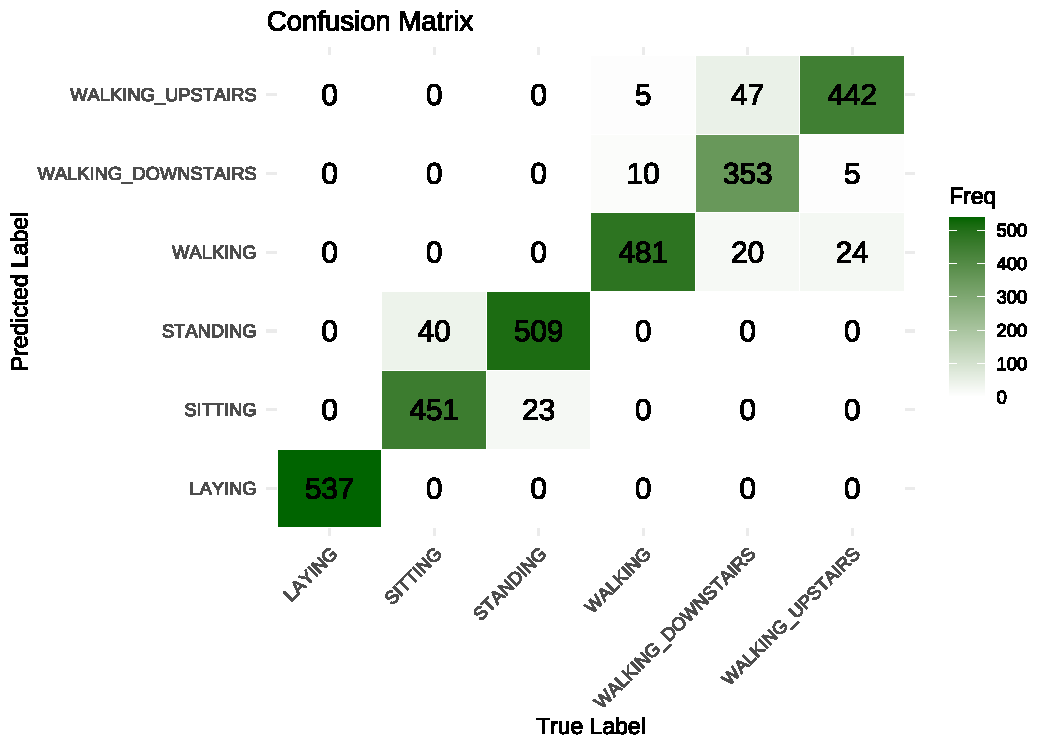
\includegraphics{report_files/figure-latex/unnamed-chunk-26-1.pdf}

\begin{Shaded}
\begin{Highlighting}[]
\CommentTok{\#install.packages("dplyr")}
\CommentTok{\#install.packages("umap")}

\CommentTok{\# Nạp thư viện}
\FunctionTok{library}\NormalTok{(dplyr)}
\FunctionTok{library}\NormalTok{(umap)}
\end{Highlighting}
\end{Shaded}

\begin{verbatim}
## Warning: package 'umap' was built under R version 4.4.3
\end{verbatim}

\begin{Shaded}
\begin{Highlighting}[]
\FunctionTok{library}\NormalTok{(ggplot2)}

\NormalTok{train\_umap }\OtherTok{\textless{}{-}}\NormalTok{ train}
\NormalTok{df\_umap }\OtherTok{\textless{}{-}}\NormalTok{ train\_umap }\SpecialCharTok{\%\textgreater{}\%} \FunctionTok{select}\NormalTok{(}\SpecialCharTok{{-}}\NormalTok{subject, }\SpecialCharTok{{-}}\NormalTok{Activity)}

\NormalTok{umap\_result }\OtherTok{\textless{}{-}} \FunctionTok{umap}\NormalTok{(df\_umap)}
\NormalTok{df\_umap\_result }\OtherTok{\textless{}{-}} \FunctionTok{as.data.frame}\NormalTok{(umap\_result}\SpecialCharTok{$}\NormalTok{layout)}
\NormalTok{df\_umap\_result}\SpecialCharTok{$}\NormalTok{Activity }\OtherTok{\textless{}{-}}\NormalTok{ train\_umap}\SpecialCharTok{$}\NormalTok{Activity}

\CommentTok{\# train\_umap}
\CommentTok{\# df\_umap\_result}
\end{Highlighting}
\end{Shaded}

Trực quan hóa kết quả giảm chiều bằng umap

\begin{Shaded}
\begin{Highlighting}[]
\FunctionTok{ggplot}\NormalTok{(df\_umap\_result, }\FunctionTok{aes}\NormalTok{(}\AttributeTok{x =}\NormalTok{ V1, }\AttributeTok{y =}\NormalTok{ V2, }\AttributeTok{color =}\NormalTok{ Activity)) }\SpecialCharTok{+}
  \FunctionTok{geom\_point}\NormalTok{(}\AttributeTok{alpha =} \FloatTok{0.7}\NormalTok{) }\SpecialCharTok{+}
  \FunctionTok{labs}\NormalTok{(}
    \AttributeTok{title =} \StringTok{"UMAP "}\NormalTok{,}
    \AttributeTok{x =} \StringTok{"UMAP1"}\NormalTok{,}
    \AttributeTok{y =} \StringTok{"UMAP2"}
\NormalTok{  ) }\SpecialCharTok{+}
  \FunctionTok{theme\_minimal}\NormalTok{(}\AttributeTok{base\_size =} \DecValTok{14}\NormalTok{) }\SpecialCharTok{+}
  \FunctionTok{theme}\NormalTok{(}\AttributeTok{plot.title =} \FunctionTok{element\_text}\NormalTok{(}\AttributeTok{hjust =} \FloatTok{0.5}\NormalTok{, }\AttributeTok{face =} \StringTok{"bold"}\NormalTok{))}
\end{Highlighting}
\end{Shaded}

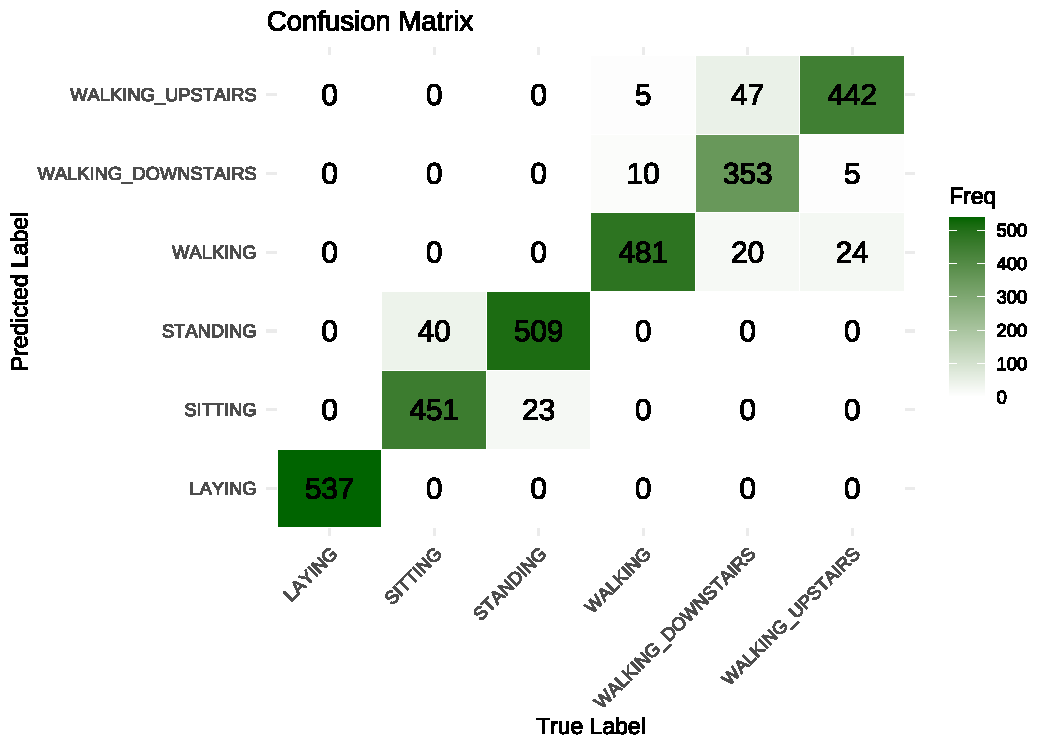
\includegraphics{report_files/figure-latex/unnamed-chunk-28-1.pdf}

Trực quan kết quả phân cụm umap với k = 2

\begin{Shaded}
\begin{Highlighting}[]
\FunctionTok{set.seed}\NormalTok{(}\DecValTok{42}\NormalTok{)}
\NormalTok{kmeans\_result }\OtherTok{\textless{}{-}} \FunctionTok{kmeans}\NormalTok{(df\_umap\_result[, }\DecValTok{1}\SpecialCharTok{:}\DecValTok{2}\NormalTok{], }\AttributeTok{centers =} \DecValTok{2}\NormalTok{, }\AttributeTok{nstart =} \DecValTok{25}\NormalTok{)}
\NormalTok{df\_umap\_result}\SpecialCharTok{$}\NormalTok{Cluster }\OtherTok{\textless{}{-}} \FunctionTok{as.factor}\NormalTok{(kmeans\_result}\SpecialCharTok{$}\NormalTok{cluster)}
\NormalTok{df\_umap\_result}\SpecialCharTok{$}\NormalTok{Label }\OtherTok{\textless{}{-}} \FunctionTok{ifelse}\NormalTok{(df\_umap\_result}\SpecialCharTok{$}\NormalTok{Cluster }\SpecialCharTok{==} \DecValTok{1}\NormalTok{, }\StringTok{"Tĩnh"}\NormalTok{, }\StringTok{"Di chuyển"}\NormalTok{)}

\FunctionTok{ggplot}\NormalTok{(df\_umap\_result, }\FunctionTok{aes}\NormalTok{(}\AttributeTok{x =}\NormalTok{ V1, }\AttributeTok{y =}\NormalTok{ V2, }\AttributeTok{color =}\NormalTok{ Label)) }\SpecialCharTok{+}
  \FunctionTok{geom\_point}\NormalTok{(}\AttributeTok{alpha =} \FloatTok{0.8}\NormalTok{, }\AttributeTok{size =} \DecValTok{2}\NormalTok{) }\SpecialCharTok{+}
  \FunctionTok{labs}\NormalTok{(}
    \AttributeTok{title =} \StringTok{"Phân cụm KMeans sau khi giảm chiều bằng UMAP"}\NormalTok{,}
    \AttributeTok{x =} \StringTok{"UMAP 1"}\NormalTok{, }\AttributeTok{y =} \StringTok{"UMAP 2"}\NormalTok{,}
    \AttributeTok{color =} \StringTok{"Ý nghĩa cụm"}
\NormalTok{  ) }\SpecialCharTok{+}
  \FunctionTok{scale\_color\_manual}\NormalTok{(}\AttributeTok{values =} \FunctionTok{c}\NormalTok{(}\StringTok{"Tĩnh"} \OtherTok{=} \StringTok{"\#E64B35"}\NormalTok{, }\StringTok{"Di chuyển"} \OtherTok{=} \StringTok{"\#00A087"}\NormalTok{)) }\SpecialCharTok{+}
  \FunctionTok{theme\_minimal}\NormalTok{(}\AttributeTok{base\_size =} \DecValTok{14}\NormalTok{) }\SpecialCharTok{+}
  \FunctionTok{theme}\NormalTok{(}\AttributeTok{plot.title =} \FunctionTok{element\_text}\NormalTok{(}\AttributeTok{hjust =} \FloatTok{0.5}\NormalTok{))}
\end{Highlighting}
\end{Shaded}

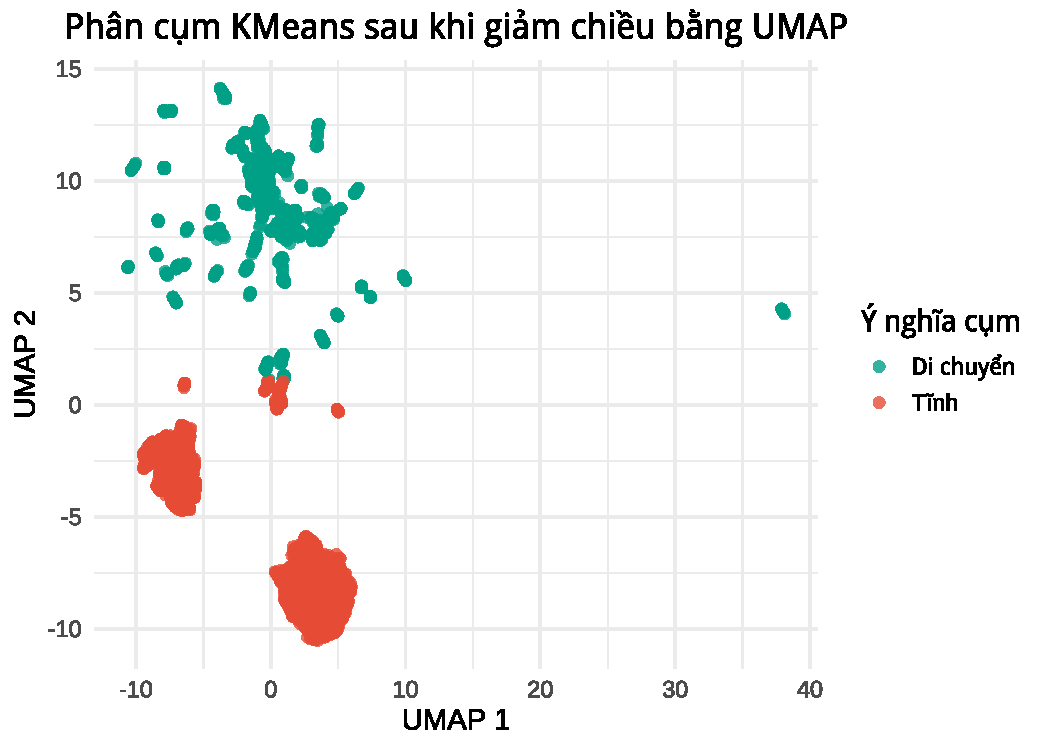
\includegraphics{report_files/figure-latex/unnamed-chunk-29-1.pdf}

\begin{Shaded}
\begin{Highlighting}[]
\CommentTok{\# install.packages("Rtsne")  \# nếu chưa cài}
\FunctionTok{library}\NormalTok{(Rtsne)}
\end{Highlighting}
\end{Shaded}

\begin{verbatim}
## Warning: package 'Rtsne' was built under R version 4.4.3
\end{verbatim}

\begin{Shaded}
\begin{Highlighting}[]
\NormalTok{train\_tsne }\OtherTok{\textless{}{-}}\NormalTok{ train}
\NormalTok{df\_tsne }\OtherTok{\textless{}{-}}\NormalTok{ train\_tsne }\SpecialCharTok{\%\textgreater{}\%} \FunctionTok{select}\NormalTok{(}\SpecialCharTok{{-}}\NormalTok{subject, }\SpecialCharTok{{-}}\NormalTok{Activity)}

\FunctionTok{set.seed}\NormalTok{(}\DecValTok{42}\NormalTok{)  }\CommentTok{\# đảm bảo tái lập kết quả}
\NormalTok{tsne\_result }\OtherTok{\textless{}{-}} \FunctionTok{Rtsne}\NormalTok{(}\FunctionTok{as.matrix}\NormalTok{(df\_tsne), }\AttributeTok{dims =} \DecValTok{2}\NormalTok{, }\AttributeTok{perplexity =} \DecValTok{30}\NormalTok{, }\AttributeTok{verbose =} \ConstantTok{TRUE}\NormalTok{, }\AttributeTok{max\_iter =} \DecValTok{500}\NormalTok{)}
\end{Highlighting}
\end{Shaded}

\begin{verbatim}
## Performing PCA
## Read the 7352 x 50 data matrix successfully!
## OpenMP is working. 1 threads.
## Using no_dims = 2, perplexity = 30.000000, and theta = 0.500000
## Computing input similarities...
## Building tree...
## Done in 2.08 seconds (sparsity = 0.017122)!
## Learning embedding...
## Iteration 50: error is 93.861229 (50 iterations in 1.29 seconds)
## Iteration 100: error is 81.745900 (50 iterations in 1.31 seconds)
## Iteration 150: error is 79.073438 (50 iterations in 0.55 seconds)
## Iteration 200: error is 78.158564 (50 iterations in 0.56 seconds)
## Iteration 250: error is 77.781913 (50 iterations in 0.56 seconds)
## Iteration 300: error is 2.660835 (50 iterations in 0.51 seconds)
## Iteration 350: error is 2.268763 (50 iterations in 0.49 seconds)
## Iteration 400: error is 2.046950 (50 iterations in 0.49 seconds)
## Iteration 450: error is 1.904216 (50 iterations in 0.49 seconds)
## Iteration 500: error is 1.804544 (50 iterations in 0.49 seconds)
## Fitting performed in 6.75 seconds.
\end{verbatim}

\begin{Shaded}
\begin{Highlighting}[]
\NormalTok{df\_tsne\_result }\OtherTok{\textless{}{-}} \FunctionTok{as.data.frame}\NormalTok{(tsne\_result}\SpecialCharTok{$}\NormalTok{Y)}
\NormalTok{df\_tsne\_result}\SpecialCharTok{$}\NormalTok{Activity }\OtherTok{\textless{}{-}}\NormalTok{ train\_tsne}\SpecialCharTok{$}\NormalTok{Activity}

\CommentTok{\# df\_tsne\_result}
\end{Highlighting}
\end{Shaded}

\begin{Shaded}
\begin{Highlighting}[]
\FunctionTok{ggplot}\NormalTok{(df\_tsne\_result, }\FunctionTok{aes}\NormalTok{(}\AttributeTok{x =}\NormalTok{ V1, }\AttributeTok{y =}\NormalTok{ V2, }\AttributeTok{color =}\NormalTok{ Activity)) }\SpecialCharTok{+}
  \FunctionTok{geom\_point}\NormalTok{(}\AttributeTok{alpha =} \FloatTok{0.7}\NormalTok{) }\SpecialCharTok{+}
  \FunctionTok{labs}\NormalTok{(}
    \AttributeTok{title =} \StringTok{"t{-}SNE "}\NormalTok{,}
    \AttributeTok{x =} \StringTok{"t{-}SNE1"}\NormalTok{,}
    \AttributeTok{y =} \StringTok{"t{-}SNE2"}
\NormalTok{  ) }\SpecialCharTok{+}
  \FunctionTok{theme\_minimal}\NormalTok{(}\AttributeTok{base\_size =} \DecValTok{14}\NormalTok{) }\SpecialCharTok{+}
  \FunctionTok{theme}\NormalTok{(}\AttributeTok{plot.title =} \FunctionTok{element\_text}\NormalTok{(}\AttributeTok{hjust =} \FloatTok{0.5}\NormalTok{, }\AttributeTok{face =} \StringTok{"bold"}\NormalTok{))}
\end{Highlighting}
\end{Shaded}

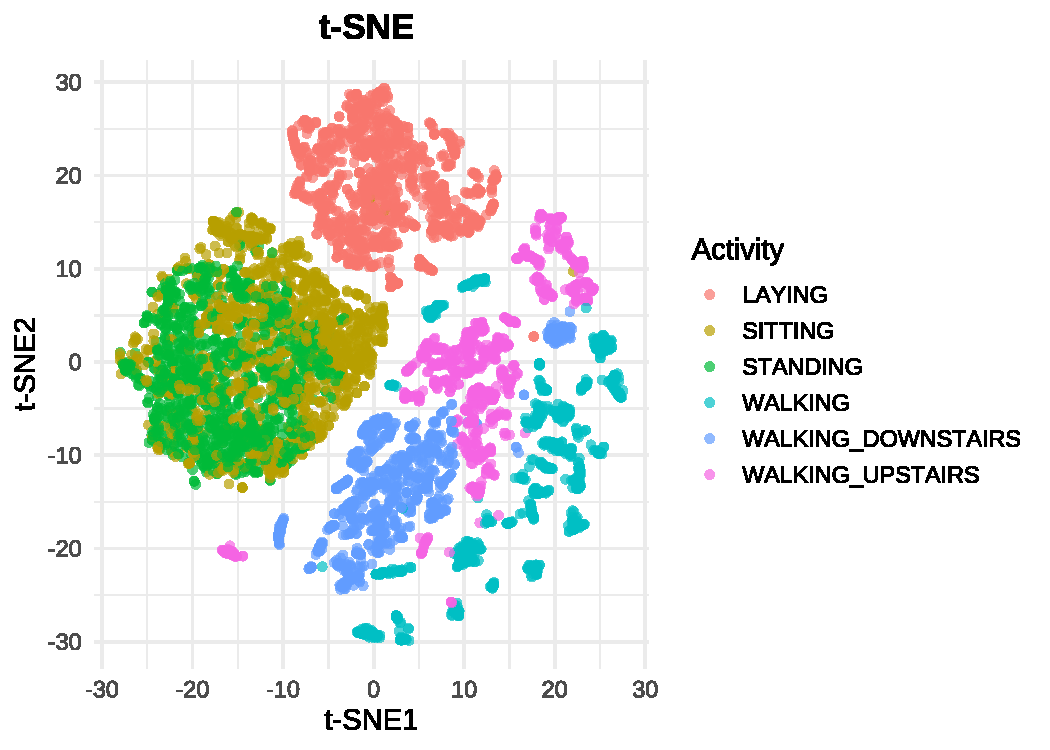
\includegraphics{report_files/figure-latex/unnamed-chunk-31-1.pdf} \#
Methodology (Phương pháp)

\end{document}
